\graphicspath{{content/chapters/3_literature/figures/}}

\chapter{Literature Review}%
\label{chp:literature}
\rule{\textwidth}{1pt} \\[1ex]

\epigraph{\textit{``We are like dwarfs sitting on the shoulders of giants.''}}{\textbf{-- Bernard of Chartres}}

\section{Introduction}
\label{sec:3_introduction}

\section{Review of Object Detection Techniques}
\label{sec:3_detection}

\subsection{Traditional Detectors}
\label{subsec:3_traditional_detectors}
\cite{od_3} SIFT, SURF, Viola Jones, etc. . .

\subsection{One-Stage Detectors}
\label{subsec:3_one-stage}

\subsubsection{OverFeat}
\label{subsubsec:3_overfeat}

\subsubsection{YOLO}
\label{subsubsec:3_yolo}
different versions based on space

\subsubsection{SSD}
\label{subsubsec:3_ssd}

\subsubsection{RetinaNet}
\label{subsubsec:3_retinanet}

\subsubsection{FCOS}
\label{subsubsec:3_fcos}

\subsubsection{YOLO-World}
\label{subsubsec:3_yolo-world}

\subsection{Two-Stage Detectors}
\label{subsec:3_two-stage}

\subsubsection{R-CNN}
\label{subsubsec:3_rcnn}

\subsubsection{Fast R-CNN}
\label{subsubsec:3_fastrcnn}

\subsubsection{Faster R-CNN}
\label{subsubsec:3_fasterrcnn}

\subsubsection{Mask R-CNN}
\label{subsubsec:3_maskrcnn}

\subsubsection{EfficientDet}
\label{subsubsec:3_efficientdet}

\subsection{Reinforcement Learning-Based Detectors}
\label{subsec:3_rl-stage}
Active Object Localisation with Deep Reinforcement Learning and \cite{bartolo2024integrating}

\subsection{Transformer-Based Detectors}
\label{subsec:3_transformer-stage}

\subsubsection{DETR}
\label{subsubsec:3_detr}

\subsubsection{Grounding DINO}
\label{subsubsec:3_groundingdino}

\subsubsection{RT-DETR}
\label{subsubsec:3_rt_detr}

\subsubsection{PaliGemma}
\label{subsubsec:3_paligemma}

\section{Review of Small Object Detection Techniques}
\label{sec:3_small_detection}

\subsection{Feature Pyramid Networks}
\label{subsec:3_fpn}

\subsection{Tiling}
\label{subsec:3_tiling}

\subsection{Focal Loss}
\label{subsec:3_focalLoss}

\subsection{Slicing Aided Hyper Inference and Fine-Tuning}
\label{subsec:3_sahi}

\section{Review of Litter Detection Approaches}
\label{sec:3_litter}

\subsection{BDW Dataset}
\label{subsec:3_bdw}

The \gls{bdw} dataset, introduced in 2018, focuses on detecting plastic bottles from diverse backgrounds using \gls{uav} imagery to facilitate recycling efforts. The dataset comprises of images captured from a DJI Phantom 4 Pro quadcopter equipped with a 3-axis stabilised gimbal. The footage was taken at \gls{agl} altitudes ranging from 10 to 30 metres, with a resolution of $5472 \times 3078$ pixels. 
To enhance diversity and simulate real-world conditions, the dataset includes images featuring eight distinct background types: bush forest land, step, flat land, sand land, wasteland, mixture, plastic stadium, and grassland, as illustrated in Figure \ref{fig:bdw}. This diversity of different backgrounds, presented as part of the dataset engineering process, accounts for the complexities associated with varied backgrounds in terms of generalising to real-world data. Furthermore, the authors highlight that the plastic bottles in the dataset are relatively small, with sizes less than $50 \times 50$ pixels, and are often transparent, which allows the background to be visible through the bottles, thereby significantly increasing the detection difficulty \cite{bdwdataset}.

\begin{figure}[!htbp]
    \centering
    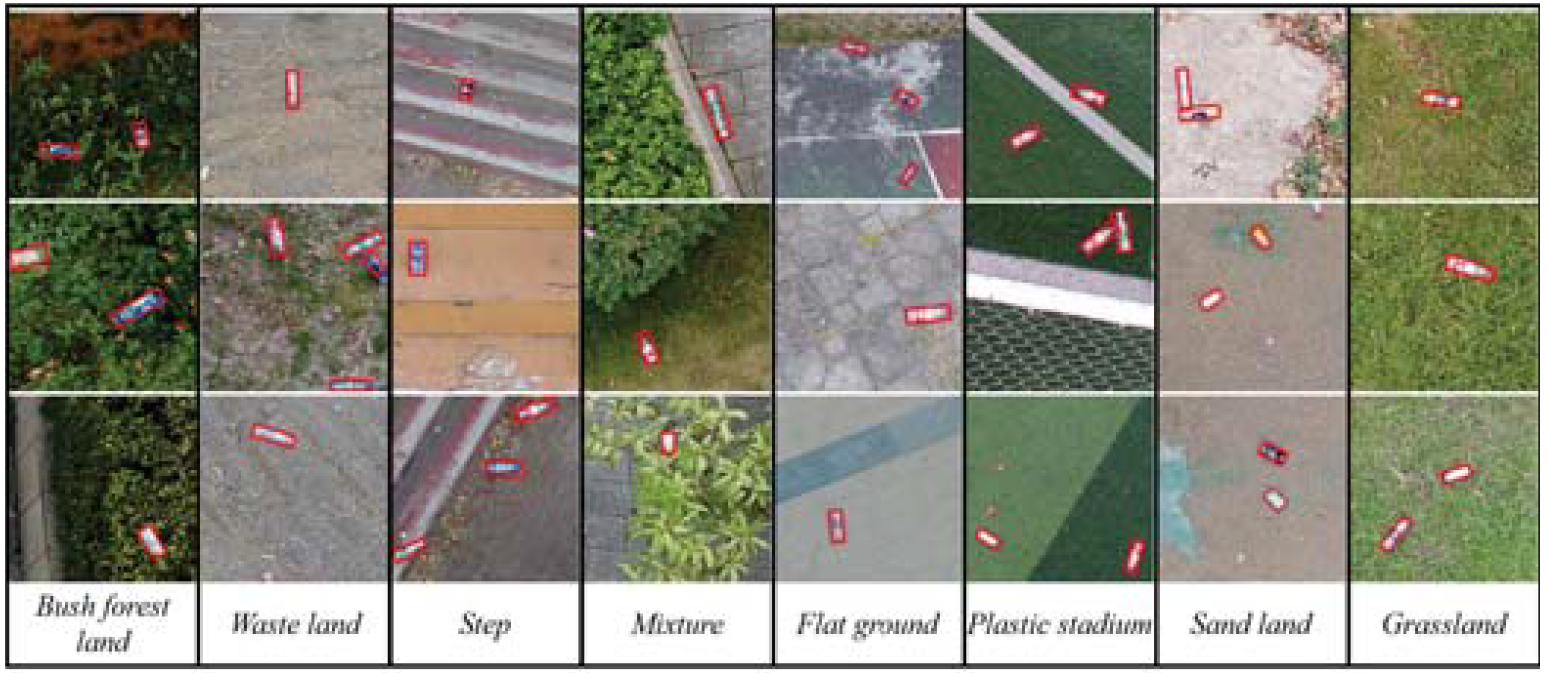
\includegraphics[width=0.9\linewidth]{BDWDataset1.png}
    \caption{Showcasing the different backgrounds found in the BDW dataset. (Source: \cite{bdwdataset})}
    \label{fig:bdw}
\end{figure}

The BDW dataset contains 25,407 annotated images with 34,791 object instances, all belonging to a single category: \textit{plastic bottles}. Annotations in the BDW dataset utilise \gls{obbs}, which include traditional bounding box coordinates along with additional parameters: centre coordinates ($c_x$, $c_y$), height ($h$), width ($w$), and orientation angle ($\theta$), where $\theta$ represents the angle from the horizontal axis. Additionally, the dataset was split randomly into training (64\%), validation (16\%), and testing (20\%) subsets \cite{bdwdataset}.

In their study, the authors utilise the created BDW dataset in multiple experiments to train object detection models, including Faster \gls{rcnn}, \gls{ssd}, \gls{yolo}v2, and a Modified \gls{rrpn} from \cite{rrpn}. Among these models, RRPN uniquely predicts OBBs, whereas the others predict standard axis-aligned bounding boxes. Wang et al. report that these experiments demonstrate that OBB regression is crucial for oriented object detection. In addition, RRPN achieved superior localisation accuracy while minimising false alarms and false positives, making it the most effective model in the study \cite{bdwdataset}.

\subsection{UM Geo. Survey}
\label{subsec:3_geosurvey}

Building on the concept of litter detection proposed by \cite{bdwdataset}, A. Deidun et al. (2018) introduced an optimised system for monitoring beach litter through aerial imagery \cite{umgeosurvey}. Their study focused on three coastal stretches within the North-East Marine Protected Area of the Maltese Islands. The monitored areas included Bahar Ic-Caghaq, which encompassed a rocky peninsula's western and eastern flanks, and Qawra Point. 
The data collection process utilised a DJI Phantom 4 Pro drone, configured with a gimbal angle of -90 degrees and flown at an \gls{agl} altitude of 30 metres. This altitude was empirically determined to balance image quality and spatial resolution, following tests conducted at heights ranging from 20 to 50 metres. Images were captured at varying ground resolutions, ranging from 2.5 to 50 centimetres per pixel, to provide detailed visual data \cite{umgeosurvey}.

The collected footage was processed using OpenDroneMap software \cite{OpenDroneMap}, which facilitated the creation of point clouds and texture maps. Georeferenced orthophoto maps with a resolution of 1 centimetre per pixel were generated using \gls{gps} metadata embedded in the \gls{exif} data of each image file. These orthophotos were subsequently tiled and visualised in Google Earth© \cite{umgeosurvey}.

\begin{figure}[!htbp]
    \centering
    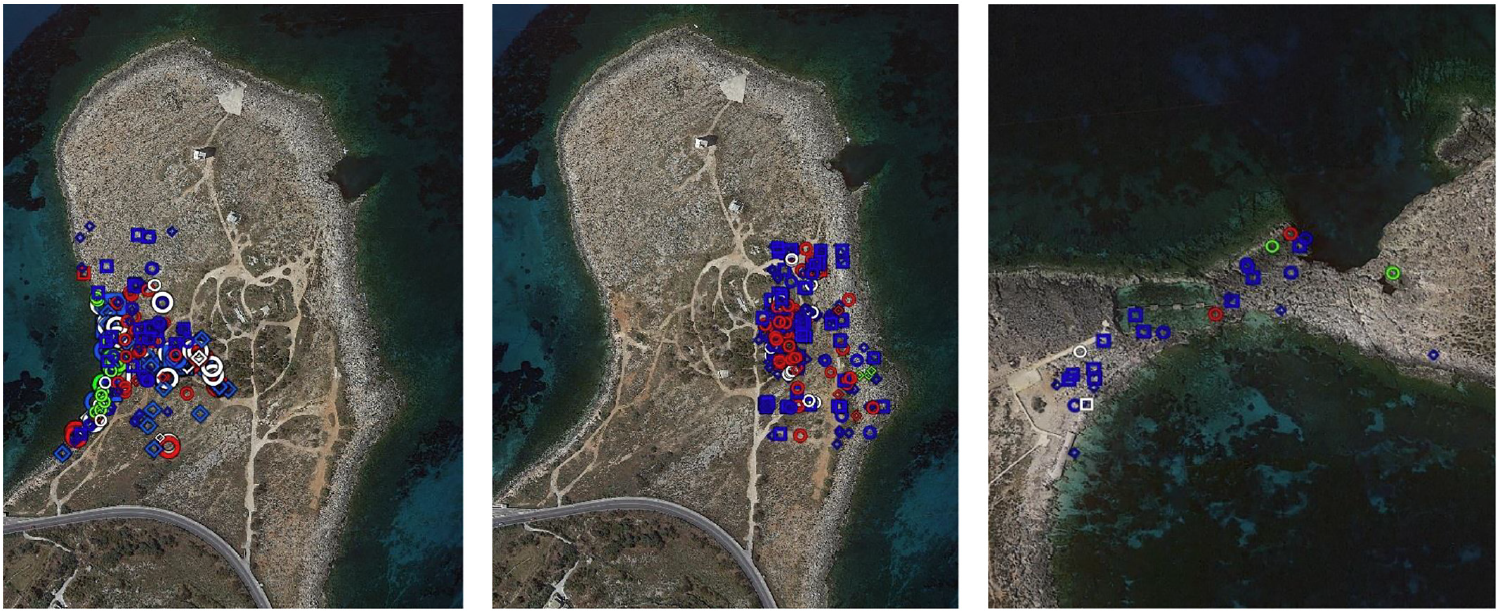
\includegraphics[width=1\linewidth]{UMgeosurvey.png}
    \caption{Showcasing snapshots from the digitised marine litter database, highlighting litter detected in the west (left) and east (middle) bays of Baħar iċ-Ċagħaq, and Qawra Point (right). Legend: blue = plastics; green = rope; red = wood; black = rubber; white = other non-natural materials. (Source: \cite{umgeosurvey})}
    \label{fig:geosurvey}
\end{figure}

The digitised database of detected marine litter, shown in Figure \ref{fig:geosurvey}, was created using 473 annotated images containing 608 labelled instances of litter. These instances were categorised into five types: \textit{plastics, rope, wood, rubber, and non-natural items}. While the study did not involve testing object detection algorithms, its key contribution lies in presenting a robust data collection protocol \cite{umgeosurvey}.

\subsection{SuperDock}
\label{subsec:3_superdock}

To address the environmental issue of trash in rivers, G. Niu et al. (2019) proposed an automated river trash monitoring system called SuperDock \cite{superdock}. This system consists of a \gls{rpu}, a docking station, and a \gls{uav}. SuperDock enables the UAV to land precisely on the docking station, where automated battery replacement is performed. This allows the UAV to resume its monitoring tasks without significant wasted time. SuperDock incorporates a deep learning-based trash detection module, leveraging the \gls{yolo}v3 architecture. As illustrated in Figure \ref{fig:superdock}, the system includes three key components: the RPU, the docking station, and the UAV. The object detection process uses data collected from a consumer-grade UAV flying at an \gls{agl} altitude of 5 to 10 meters \cite{superdock}.

\begin{figure}[!htbp]
    \centering
    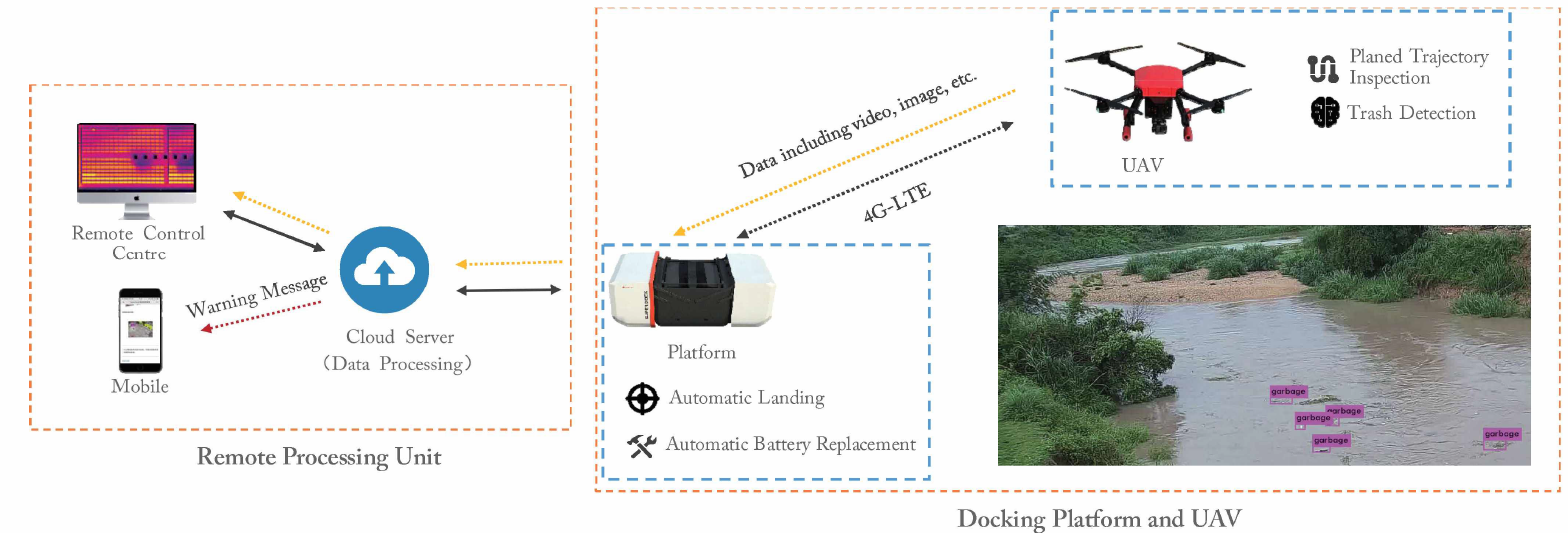
\includegraphics[width=0.9\linewidth]{superdock.png}
    \caption{Block diagram of the automated SuperDock system. (Source: \cite{superdock})}
    \label{fig:superdock}
\end{figure}

The dataset features 100 annotated images, divided into 80\% for training and 20\% for testing, with a total of 312 object instances. All types of litter in the dataset are annotated under a single category: \textit{garbage}. Data augmentation techniques were applied, increasing the dataset size by a factor of five. Additionally, the authors used Microsoft AirSim (Aerial Informatics and Robotics Simulation) to experiment with the gathered data. The dataset was used to train and test three models: Faster \gls{rcnn}, \gls{yolo}v3, and \gls{yolo}v3 with an improved loss function. Among these, the improved \gls{yolo}v3 model demonstrated the best performance in terms of both accuracy and processing time. While the study did not focus on creating a specialised litter detection dataset, its primary contribution lies in developing an automated trash monitoring system \cite{superdock}.

\subsection{Styrofoam Monitoring}
\label{subsec:3_styrofoam}
To analyse the patterns of waste generation and distribution, as well as the factors contributing to its inflow, S. H. Bak et al. (2019) proposed an automated floating trash monitoring system based on deep learning \cite{styrofoam}. Their study focused on Heungnam Beach in Geoje, situated in Korea’s marine climate zone on the South Sea. The system utilises SegNet \cite{segnet}, an instance segmentation model based on a convolutional encoder-decoder structure developed by the University of Cambridge, to detect beach litter.
While the authors did not specify the exact number of annotated images in the dataset, UAV imagery was collected using DJI's MAVIC 2 PRO, a multi-rotor UAV. The UAV operated at an altitude of 15 meters, chosen to account for the size of the beach litter and the \gls{gsd}. Orthoimages were generated using Pix4D and divided into $224 \times 224$-pixel segments for neural network input, with positional information recorded for each segment \cite{styrofoam}.

\begin{figure}[!htbp]
    \centering
    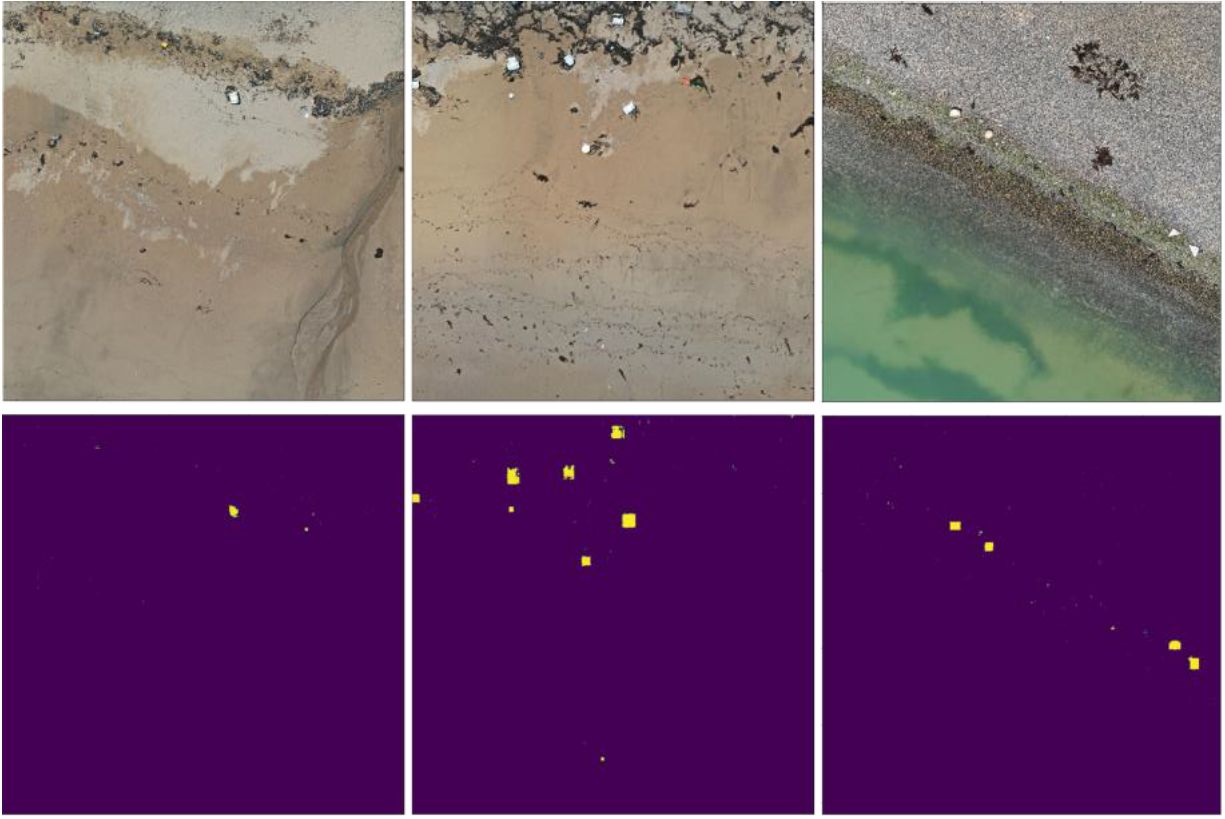
\includegraphics[width=0.7\linewidth]{styrofoam.png}
    \caption{Styrofoam detection results using the trained neural network. (Source: \cite{styrofoam})}
    \label{fig:styrofoam}
\end{figure}

The developed dataset only contained a single litter category, focusing on detecting \textit{Styrofoam} waste, and was notably imbalanced, as the majority of pixels represented the background, with less than 5\% occupied by detected objects. To mitigate this imbalance, data augmentation techniques were employed. Despite these challenges, the system achieved an impressive detection accuracy of 98.2\%, demonstrating its efficacy in identifying Styrofoam litter on beaches, as depicted in Figure \ref{fig:styrofoam} \cite{styrofoam}.

\subsection{Small Litter Detection}
\label{subsec:3_smalldetection}

In 2019, M. Schembri and D. Seychell proposed a case study focusing on litter detection through aerial imagery to address challenges in small object detection in highly variable backgrounds \cite{small_litter_detection}. This study explored techniques for small object localisation using \gls{cnn} to detect litter in outdoor, non-urban imagery. The dataset for this research was collected using a consumer-grade UAVs at altitudes ranging from 5 to 10 metres \gls{agl}. Compiled from land surveys conducted within the Maltese Islands, the dataset includes 744 annotated images with all types of litter objects classified under a single \textit{litter} category \cite{small_litter_detection}.

The authors proposed an algorithmic pipeline for small litter detection, as illustrated in Figure \ref{fig:smalllitterdetection}. A sliding window technique was used to subdivide the entire scene into tiles of $224 \times 224$ pixels with a 32-pixel overlap, and each tile was processed individually. Non-relevant objects such as the sky, sea, and humans were masked during a scene filtering stage to enhance accuracy. The litter detection problem was tackled using a VGG-16 CNN model, pre-trained on ImageNet, and fine-tuned with the collected dataset. Data augmentation techniques were also applied to improve the model’s robustness \cite{small_litter_detection}.

\begin{figure}[!htbp]
    \centering
    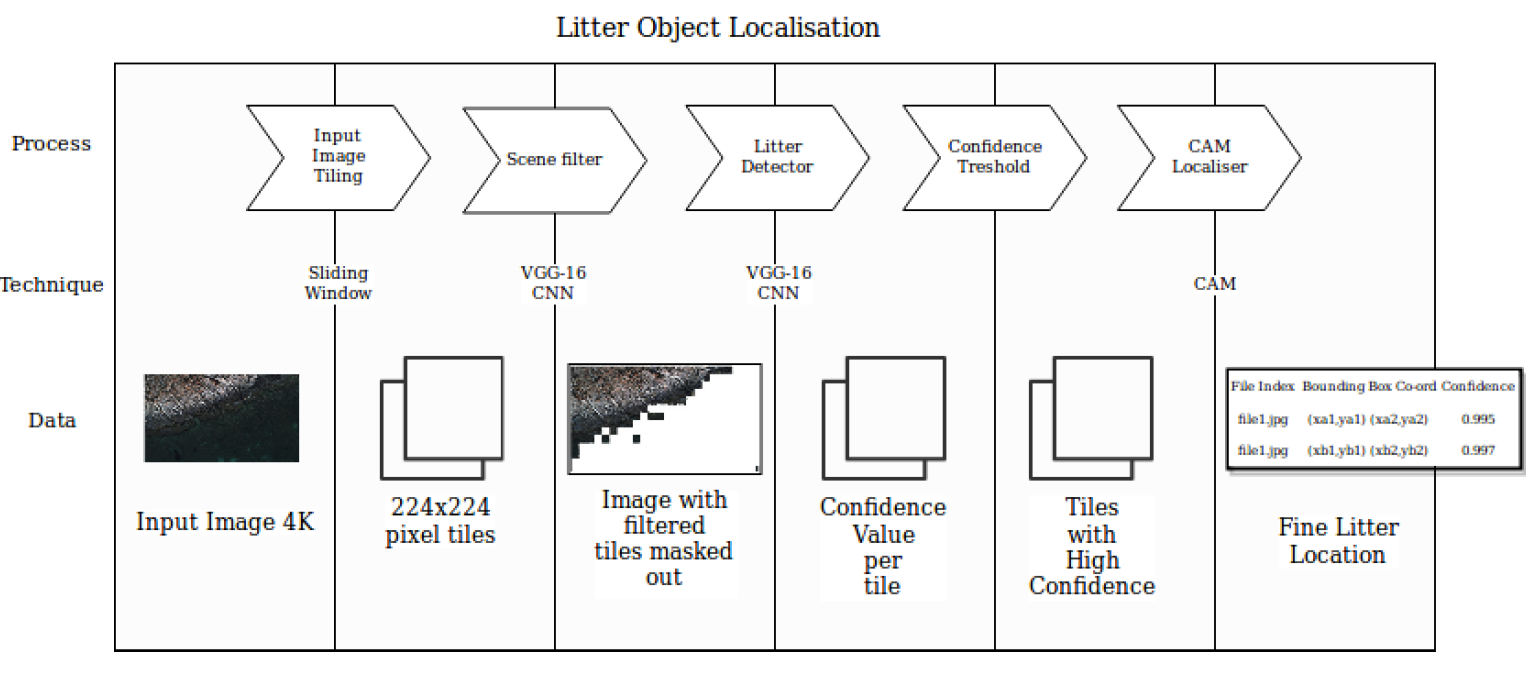
\includegraphics[width=0.9\linewidth]{small_litter_detection.png}
    \caption{Data flow and process diagram of the litter detection algorithm. (Source: \cite{small_litter_detection})}
    \label{fig:smalllitterdetection}
\end{figure}

Due to the dataset’s foreground-to-background sample ratio of 1:20, a confidence threshold was used to refine the detection results. \gls{cam} was employed to improve the \gls{iou} score by highlighting relevant foreground areas. Thresholding and normalising the heatmap allowed for generating masks that effectively located the target objects. An IoU threshold of 0.01 for \gls{nms} was used to facilitate the detection of very small objects.
The study identified that stones and vegetation were among the classes frequently misclassified as litter. To address this issue, the authors proposed a two-stage model incorporating a terrain filter to automate the detection of misclassifications, which provided improved results. They also concluded that litter with more defined shapes was easier to detect for both human annotation and algorithmic detection. 
The authors also trained Faster \gls{rcnn} on the same dataset and observed lower performance metrics, which were attributed to its difficulty in handling highly variable background representations \cite{small_litter_detection}.

\subsection{TACO Dataset}
\label{subsec:3_tacodataset}

Detecting litter in natural environments presents considerable challenges due to the variability of litter, which can be deformable, transparent, aged, fragmented, occluded, and camouflaged. Additionally, models must contend with the wide variety of features found in natural landscapes. To tackle these issues, P. F. Proença and P. Simões introduced the \gls{taco} dataset in 2020 \cite{taco2020}. This dataset was created to feature images captured from a variety of global environments, as shown in Figure \ref{fig:taco1}, including beaches and urban areas, with litter segmented and annotated according to a hierarchical classification system \cite{taco2020}.

\begin{figure}[!htbp]
    \centering
    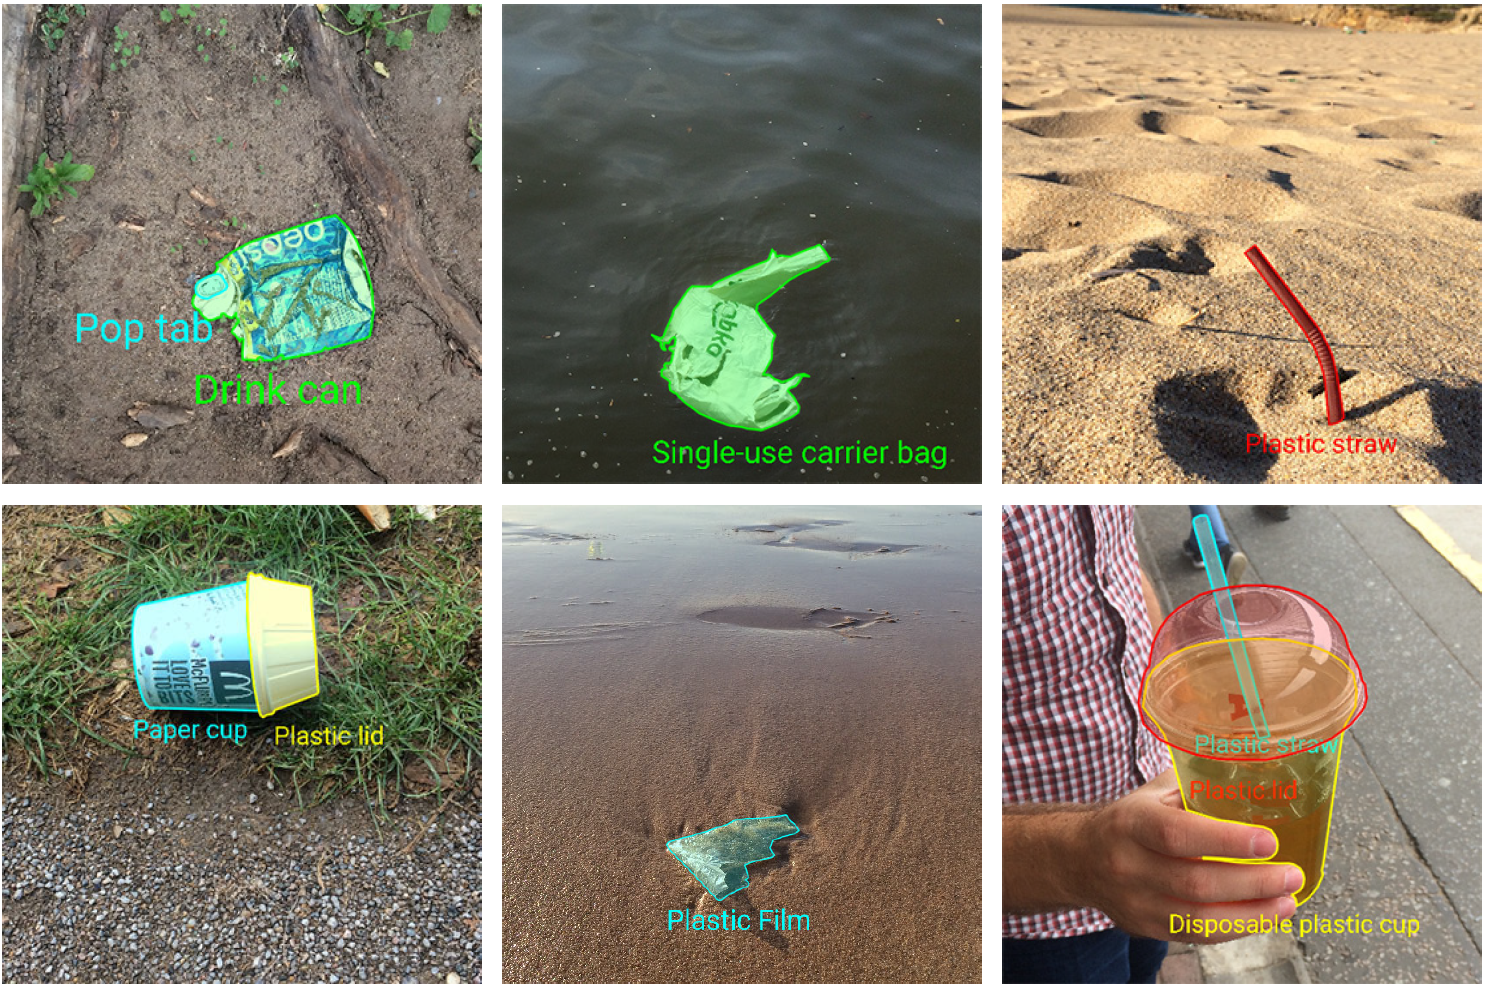
\includegraphics[width=0.8\linewidth]{taco1.png}
    \caption{Annotated images from the \gls{taco} dataset, with litter objects marked using polygon masks for instance segmentation. (Source: \cite{taco2020})}
    \label{fig:taco1}
\end{figure}

The \gls{taco} dataset includes 60 distinct litter categories, organised into 28 top-level categories, as observed in Figure \ref{fig:taco2}. Unlike UAV-based datasets, \gls{taco} consists of images captured from ground-level natural environments. At the time of release, the dataset comprised 1,500 annotated images and 4,784 instances of litter, with an additional 3,918 new images currently awaiting annotation. The dataset uses polygon masks for annotation in an attempt to tackle the problem of instance segmentation \cite{taco2020}.
The authors conducted several experiments using Mask \gls{rcnn} to evaluate the dataset's performance. Two configurations were tested:
\begin{itemize}
    \item \textbf{\gls{taco}-1:} Identifying a single class of litter.
    \item \textbf{\gls{taco}-10:} Identifying ten distinct litter classes.
\end{itemize}

\begin{figure}[ht]
    \centering
    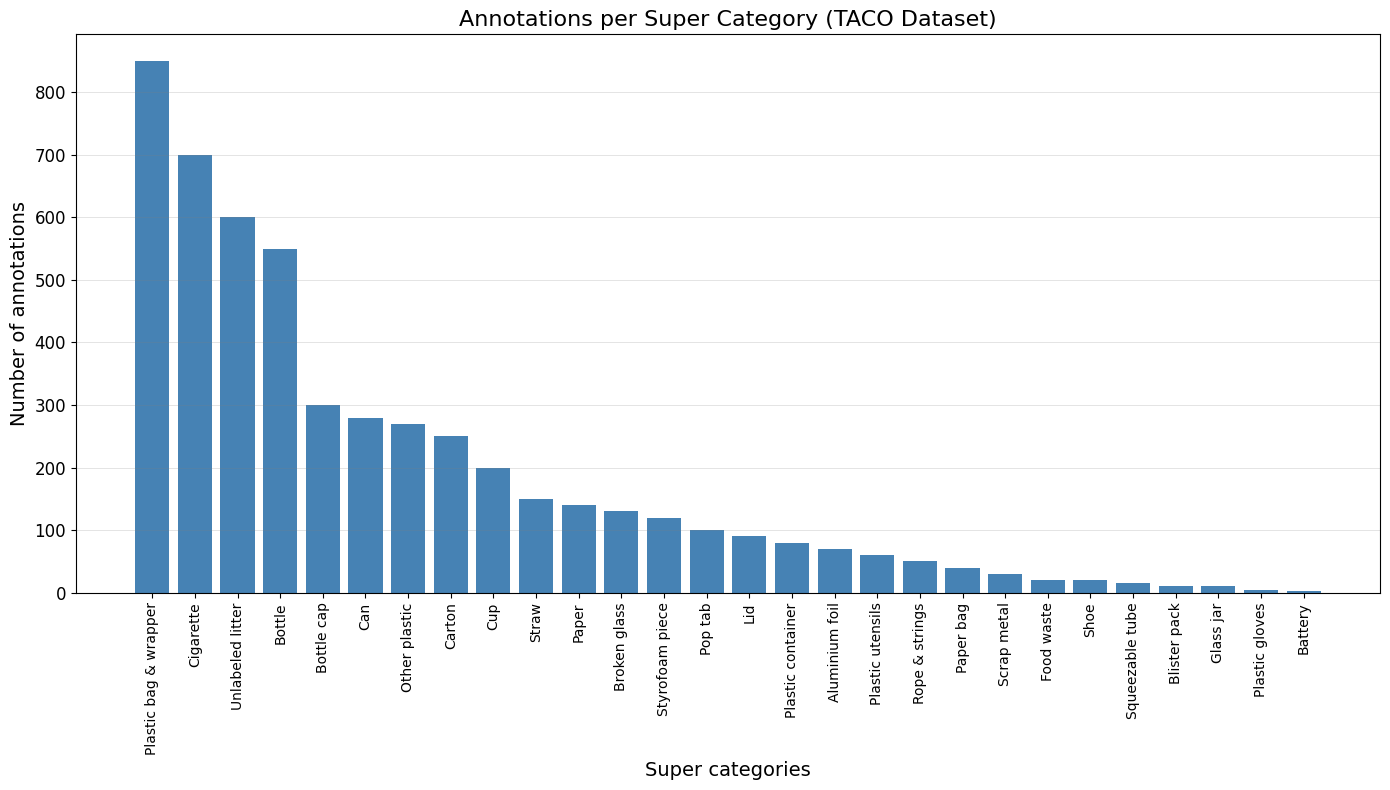
\includegraphics[width=0.7\linewidth]{taco2.png}
    \caption{Number of annotations per super category in the published version of the \gls{taco} dataset. (Source: \cite{taco2020})}
    \label{fig:taco2}
\end{figure}

The authors noted that the detection performance was notably low due to challenges in detecting small items, particularly cigarette butts, which led to a high rate of false positives and negatives. This was attributed to their small size, with most images resized to $1024 \times 1024$ pixels, causing many small objects (less than $20 \times 20$ pixels) to be missed. Larger objects, such as cans and bottles, were detected more accurately, though a considerable number of bottles were misclassified as cans. Confusion was also observed between \textit{plastic bags} and \textit{other litter}, which is understandable given the material similarities between these categories \cite{taco2020}.

\subsection{MJU-Waste Dataset}
\label{subsec:3_mju-waste}

In 2020, T. Wang et al. also sought to address the challenge of waste object segmentation through a multi-level approach \cite{mju_waste}. To create their dataset, the authors collected waste items from a university campus, photographed individuals holding these items, and then annotated the images. The MJU-Waste dataset focuses solely on a single category, classifying all items under the label of \textit{waste}. The MJU-Waste dataset contains 2,475 annotated images and 2,525 instances of litter, all of which are annotated using polygon masks.
Unlike UAV-based datasets, the MJU-Waste dataset consists of images captured from controlled environments. The dataset includes segmentation masks, along with both raw and processed depth maps for all litter instances, captured using a Microsoft Kinect RGBD camera. However, due to sensor limitations, the depth frames contain missing values, particularly at reflective surfaces, occlusion boundaries, and distant regions. To address this, a median filter was applied to fill in the missing data and ensure the depth images were of high quality. Each image in the dataset was annotated with pixel-wise masks of the waste objects, and examples of colour frames, ground-truth annotations, and depth frames are provided in Figure \ref{fig:mjuwaste}. Alongside the semantic segmentation ground truths, object instance masks are also available \cite{mju_waste}.

\begin{figure}[!htbp]
    \centering
    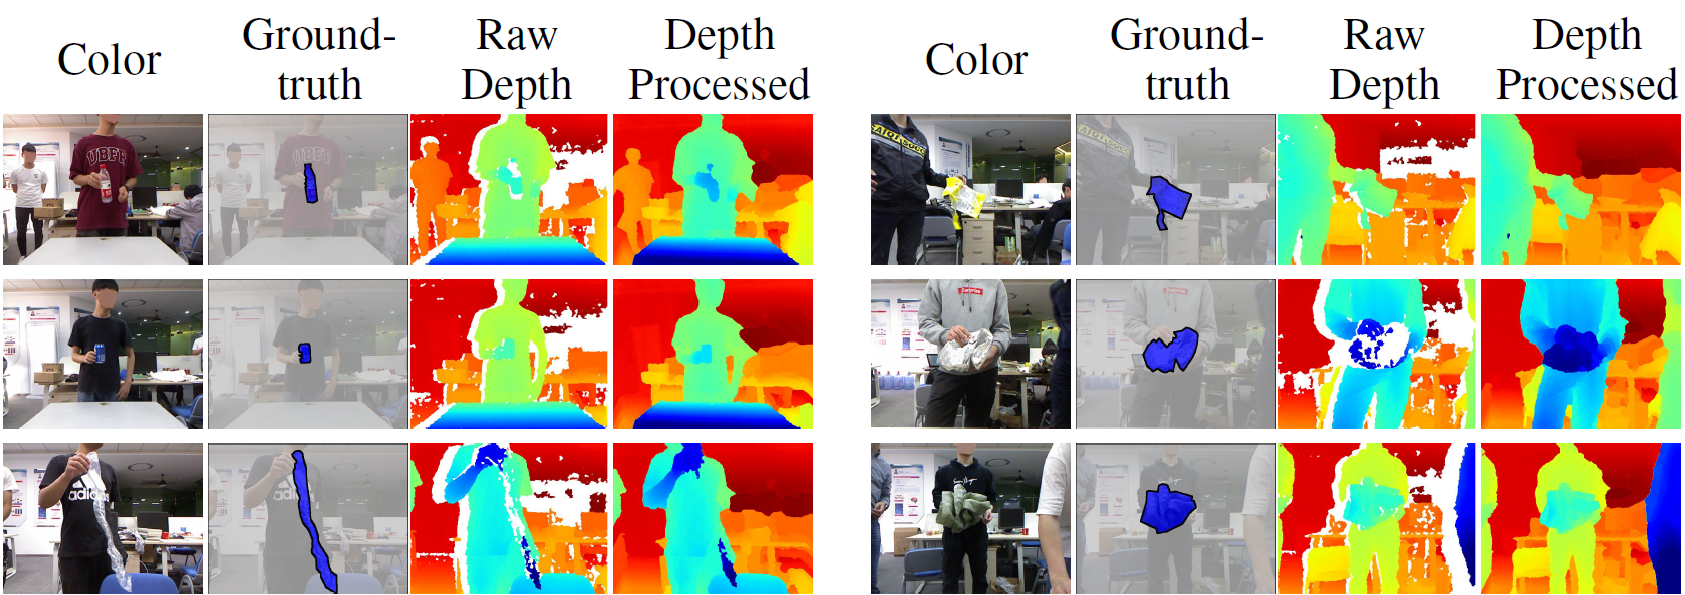
\includegraphics[width=1\linewidth]{mjuwaste.png}
    \caption{Sample RGB images, ground-truth annotations, and depth frames from the MJU-Waste dataset. (Source: \cite{mju_waste})}
    \label{fig:mjuwaste}
\end{figure}

The authors evaluate their proposed method against state-of-the-art semantic segmentation baselines. Their approach adopts a multi-level strategy for waste object segmentation, involving three key stages: first, scene-level parsing for initial coarse segmentation; second, object-level parsing to refine object region proposals; and third, pixel-level refinement using colour, depth, and spatial affinities. By combining inference from all three levels, the method achieves a coherent and accurate final segmentation.
In addition, the study focuses on two particularly challenging scenarios for waste object localisation: the hand-held setting, which is crucial for applications such as service robot interactions and smart trash bins, and waste objects found in natural environments. A significant challenge noted by the authors in both cases is the extreme variation in object scale, which leads to suboptimal performance from standard segmentation algorithms \cite{mju_waste}.

In comparison to the \gls{taco} dataset, the MJU-Waste dataset is split as follows: 60\% for training, 10\% for validation, and 30\% for testing. The evaluation metrics used include \gls{iou}, mean \gls{iou}, and pixel precision. The models tested include FCN-8s \cite{fcn}, PSPNet \cite{pspnet}, CCNet \cite{ccnet}, and DeepLabv3 \cite{deeplabv3}. Among these, DeepLabv3 performed best in terms of IoU and mIoU, while CCNet excelled in pixel precision. Notably, DeepLabv3 also outperformed other models when tested on the \gls{taco} dataset.
The authors also conclude that their multi-level approach proved effective, with scene-level segmentation, object-level segmentation, and pixel-level refinement working together to produce high-quality localisation results \cite{mju_waste}.

\subsection{UAVVaste}
\label{subsec:3_uavvaste}

In 2021, M. Kraft et al. addressed the challenge of detecting litter and the associated issue of mapping detected litter geographically \cite{uavvaste}. Their proposed system employed a \gls{uav} equipped with onboard sensors to process low-altitude aerial imagery. A key feature of the system was its reliance on low-cost, commercially available components, which were integrated into a self-contained solution capable of autonomous operation during UAV patrol missions.
A notable contribution of their research was the introduction of an application-specific dataset, UAVVaste. This dataset consists of 772 images with 3,716 bounding box annotations, as illustrated in Figure \ref{fig:uavvaste1}, and is dedicated to a single category: litter, labelled as \textit{rubbish}. The creation of this dataset was motivated by the lack of domain-specific data tailored to UAV-based litter detection. Compared to the \gls{taco} dataset, the UAVVaste dataset features a marked distribution shift, characterised by smaller object sizes, reflecting the unique challenges of detecting litter in aerial imagery \cite{uavvaste}.

\begin{figure}[!htbp]
    \centering
    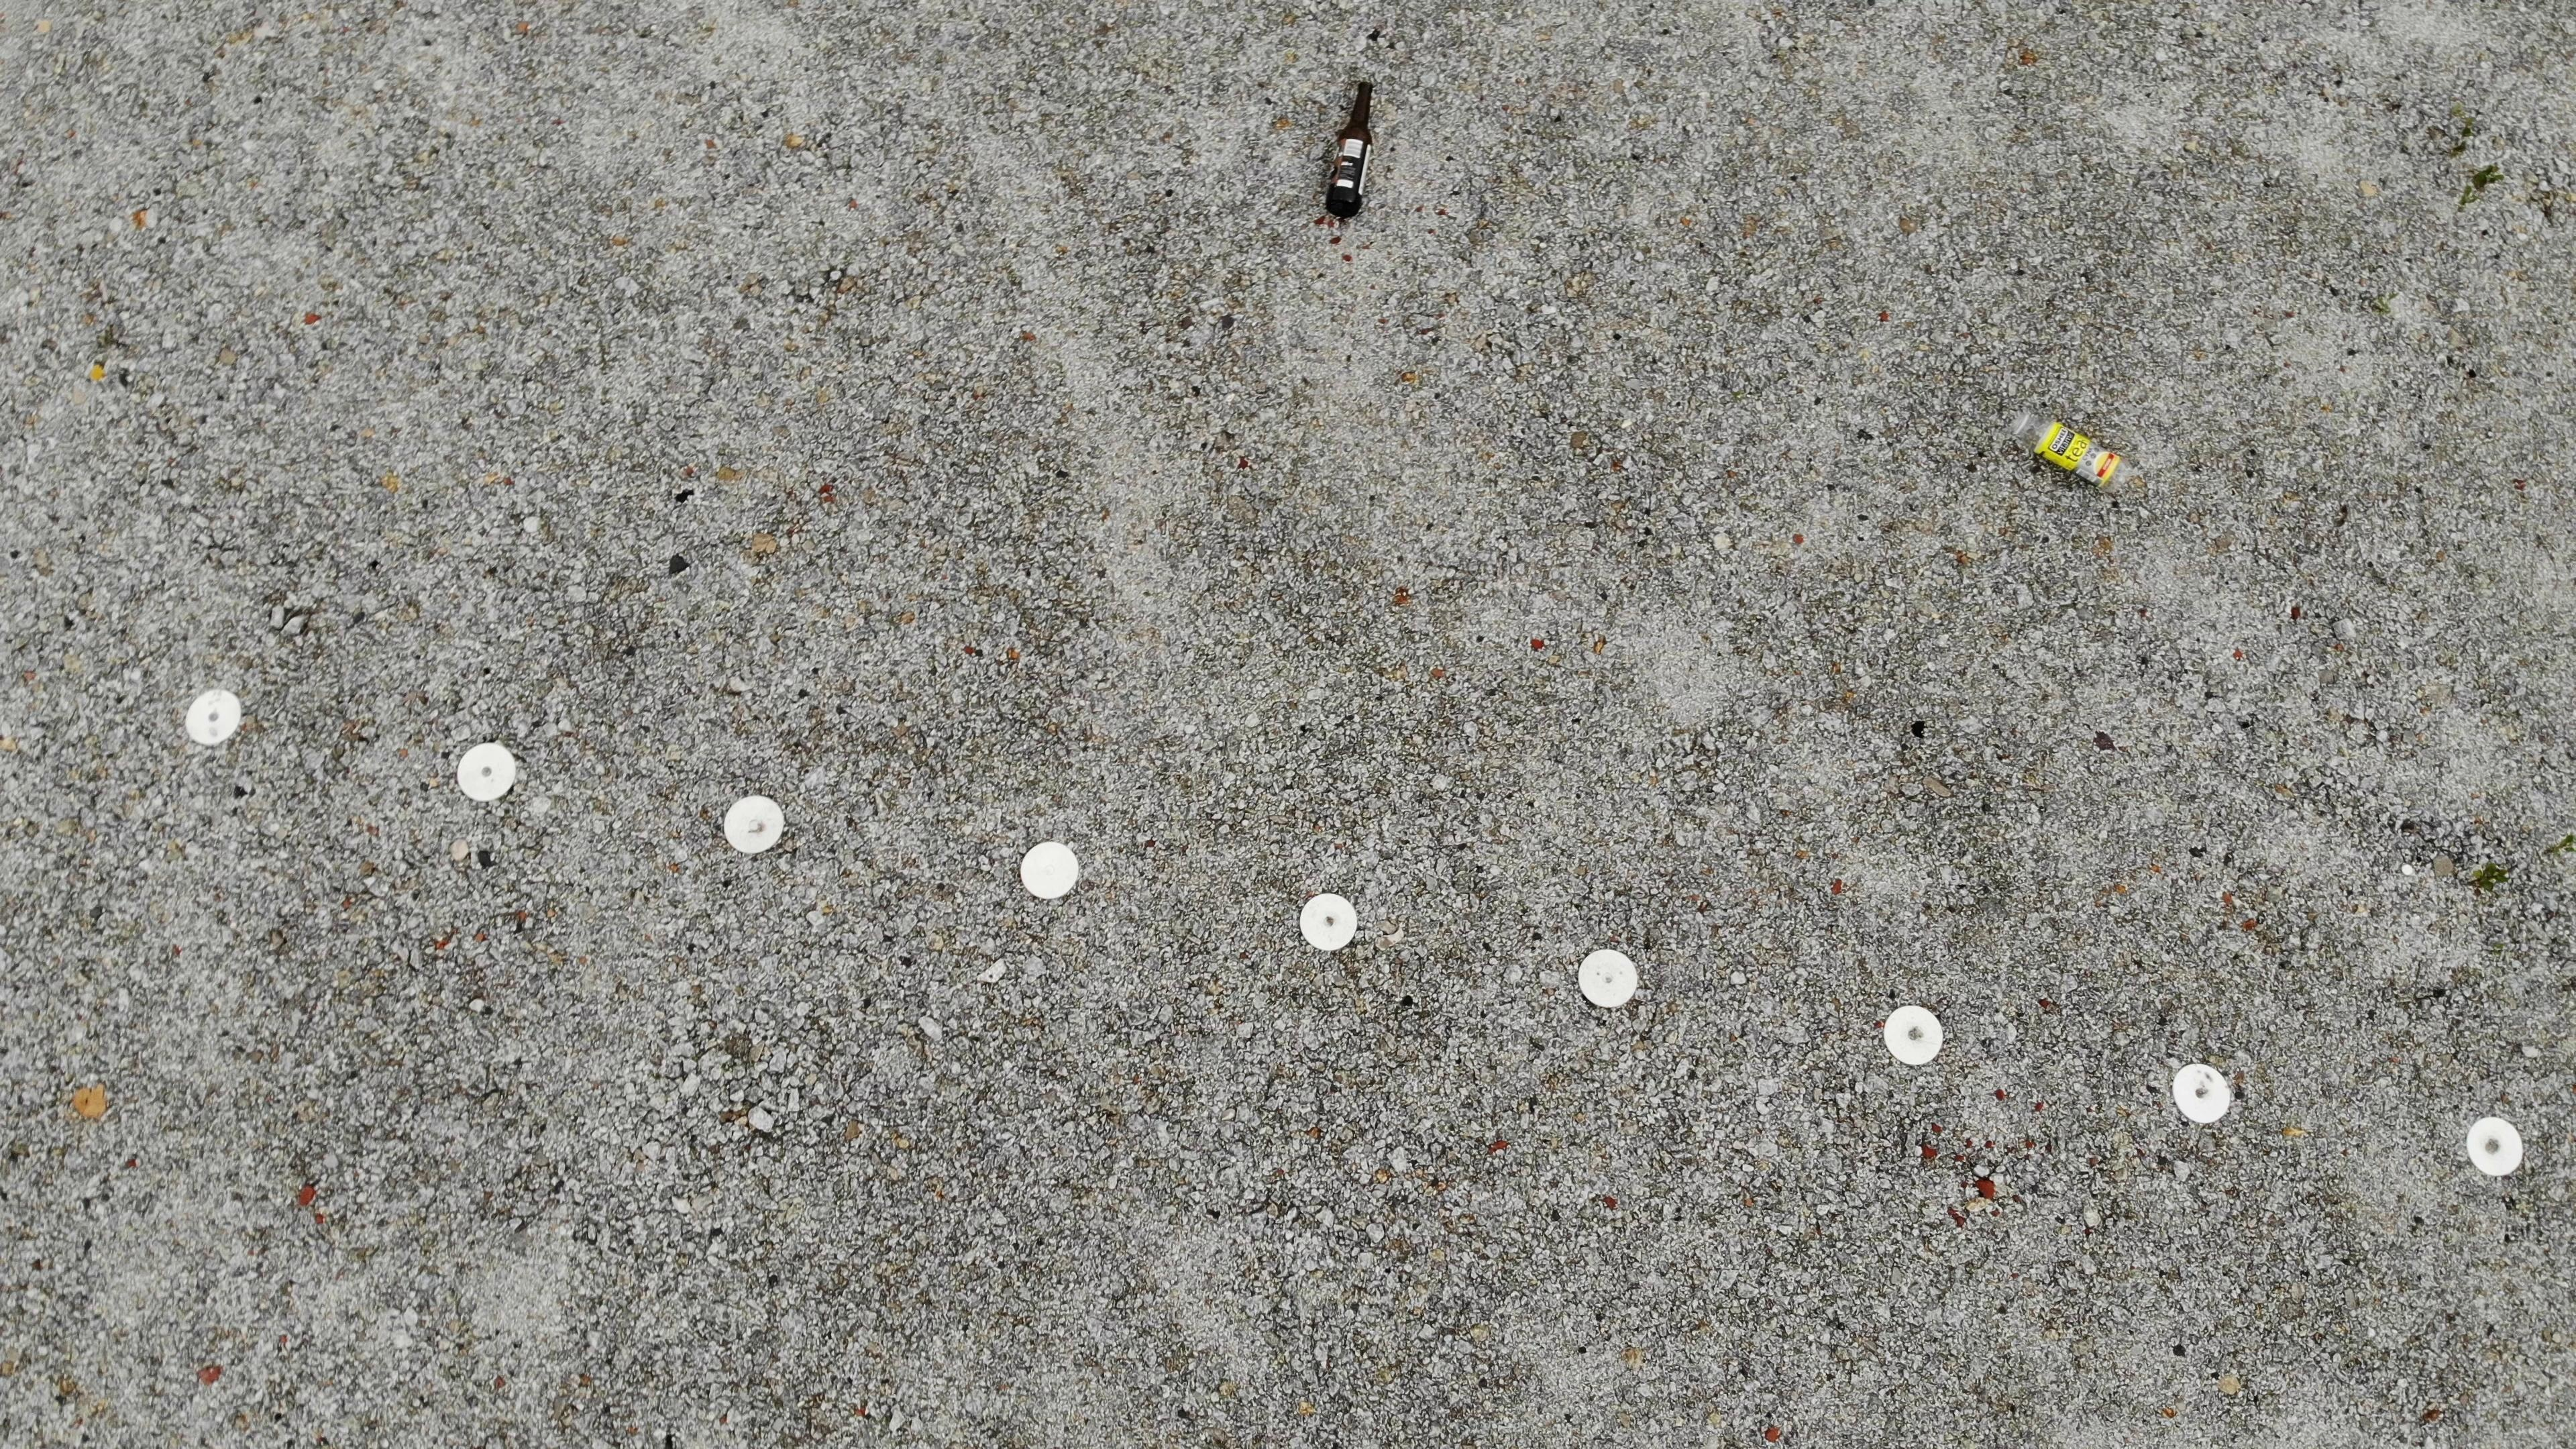
\includegraphics[width=0.9\linewidth]{uavvaste1.png}
    \caption{Sample images from the UAVVaste dataset with litter objects annotated using bounding boxes. (Source: \cite{uavvaste})}
    \label{fig:uavvaste1}
\end{figure}

The UAV hardware used in the study included a Pixhawk 2 autopilot controller, a Here2 \gls{gps}/\gls{gnss} module equipped with a barometric pressure sensor, and a downward-facing camera stabilised using a gimbal. The computational platform featured multiple components, including an Nvidia Xavier NX, a Google Coral USB (\gls{tpu}), and a Raspberry Pi 4. A variety of neural network architectures were evaluated for litter detection. These included \gls{ssd} detectors with lightweight backends optimised for TensorFlow Lite, which operated efficiently on the Google Coral TPU, as well as \gls{yolo}v3 and \gls{yolo}v4 and their lightweight variants. For models deployed on the Nvidia Xavier NX, TensorRT was utilised to optimise performance. Additionally, EfficientDet with a MobileNet backend was implemented. Training these models involved transfer learning, leveraging pre-trained weights from the \gls{coco} dataset to improve performance \cite{uavvaste}.

\begin{figure}[!htbp]
    \centering
    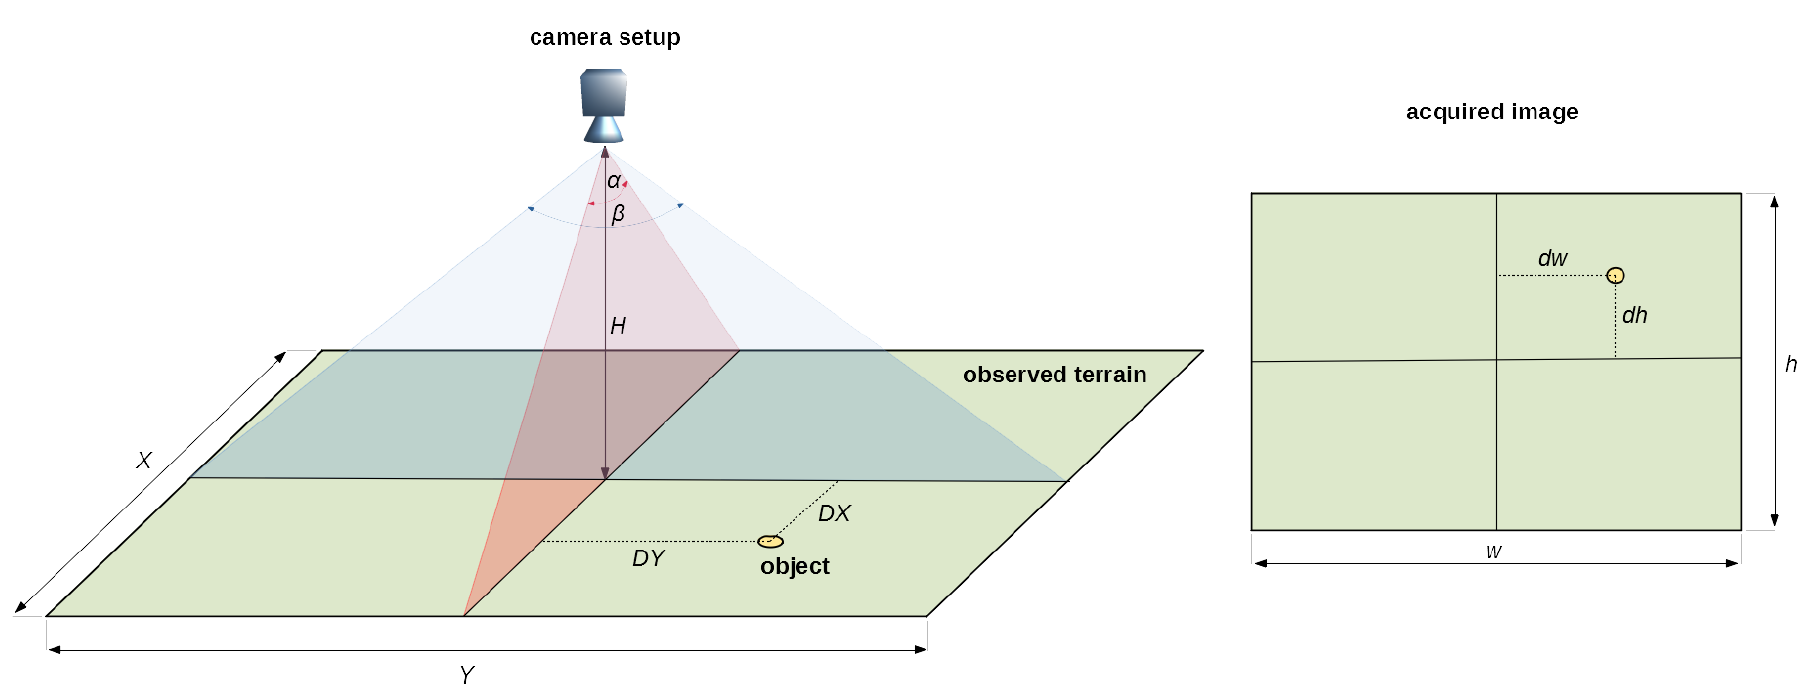
\includegraphics[width=0.9\linewidth]{uavvaste2.png}
    \caption{A schematic representation of the camera setup and acquired image, along with the key parameters. (Source: \cite{uavvaste})}
    \label{fig:uavvaste2}
\end{figure}

A significant portion of the study focused on the geolocation algorithm, which marks detected litter objects on a map using the UAV’s onboard sensors. This process required camera calibration, performed using the Kalibr library, and lens distortion correction, ensuring accurate geometric relationships between the image and real-world coordinates. The algorithm assumed a vertical downward orientation for the camera during operation. Using the known viewing angles of the camera and the UAV’s altitude, the algorithm calculated the size of the area captured in each image. Figure \ref{fig:uavvaste2} provides a schematic representation of the camera setup and the acquired image, highlighting the key parameters involved in the process. While the camera parameters were determined with high precision, the accuracy of object localisation on the map was predominantly influenced by the accuracy of altitude measurements. The authors observed that any error in altitude measurement would proportionally affect the localisation accuracy.
The evaluation metrics used in the study included the \gls{map} scores from the \gls{coco} dataset, calculated at \gls{iou} thresholds of 0.5 and 0.95. Separate \gls{map} and recall scores were also reported for small, medium, and large objects. Among the models tested, \gls{yolo}v4 achieved the highest \gls{map}, while EfficientDet excelled in recall, particularly for smaller objects \cite{uavvaste}.

\subsection{ZeroWaste Dataset}
\label{subsec:3_zerowaste}

In 2022, D. Bashkirova et al. introduced the first industrial-grade, in-the-wild waste detection and segmentation dataset, ZeroWaste, making a significant contribution to computer-aided waste detection \cite{zerowaste}. The dataset features four categories of litter: \textit{cardboard}, \textit{soft plastic}, \textit{rigid plastic}, and \textit{metal}. Unlike UAV-based datasets, the images in ZeroWaste were captured in real-world settings.
The ZeroWaste dataset includes 10,715 annotated images, collected from a high-quality paper conveyor at a single-stream recycling facility in Massachusetts, containing 27,744 instances of litter, all annotated in polygon format, as illustrated in Figure \ref{fig:zerowaste}. Data augmentation was also applied to the dataset to improve model generalisation by artificially increasing the variety of training samples. Furthermore, this four-class labelled dataset captures various waste items identified during the sorting process at the facility, which aims to separate high-quality paper from contaminants such as metal, plastic, brown paper, and cardboard \cite{zerowaste}.

\begin{figure}[!htbp]
    \centering
    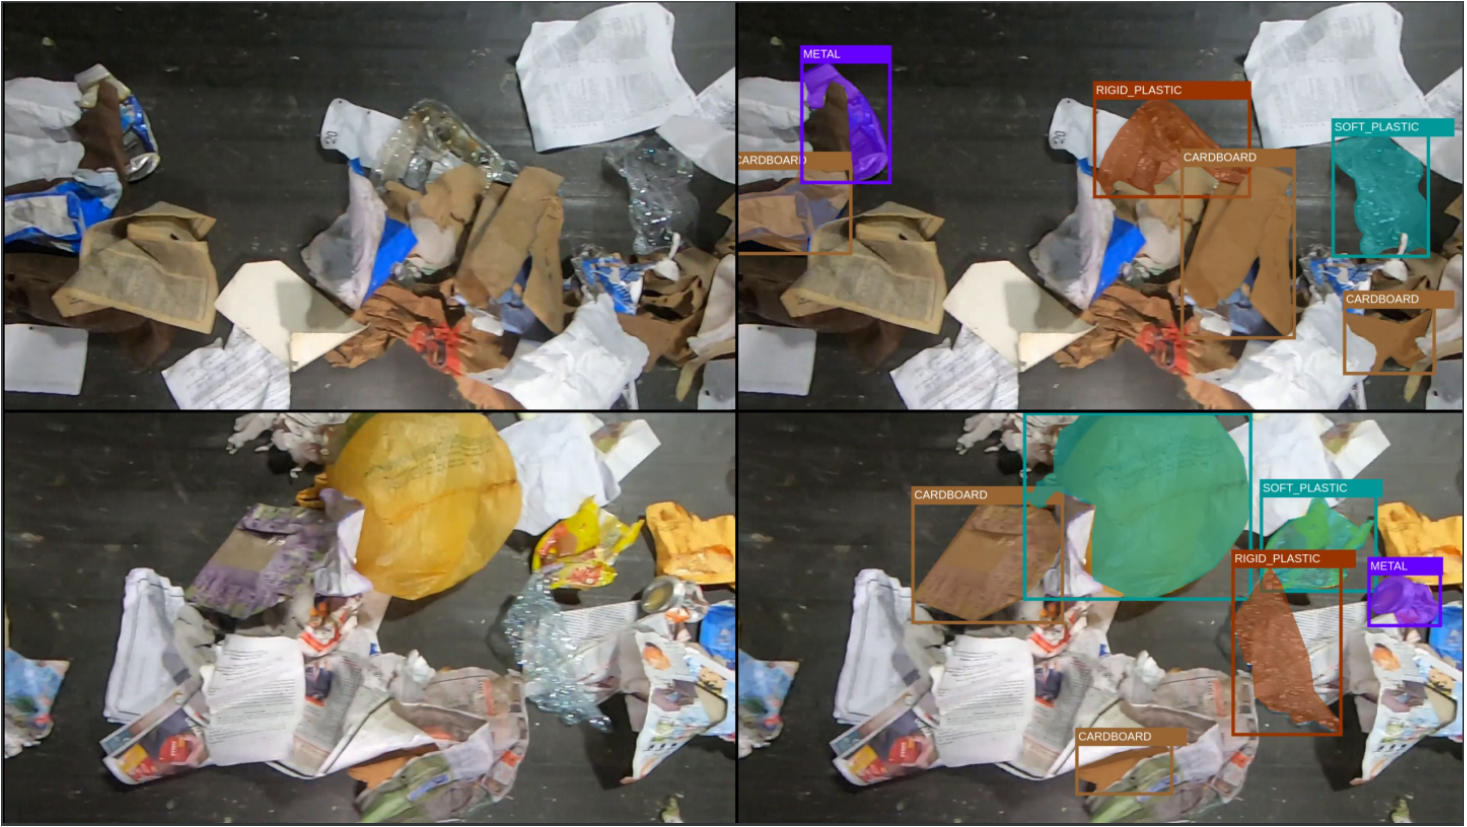
\includegraphics[width=0.9\linewidth]{zerowaste.png}
    \caption{Sample images (left) and ground truth polygon annotations (right) in the ZeroWaste dataset. (Source: \cite{zerowaste})}
    \label{fig:zerowaste}
\end{figure}

The data was gathered using two compact recording systems placed at the start and end of the conveyor belt during the facility's routine operations. The footage consists of 12 video sequences with a total duration of 95 minutes and 14 seconds, recorded at a frame rate of 120 FPS and a resolution of $1920 \times 1080$. To ensure high-quality data, the footage was processed to correct optical distortions, crop unnecessary elements, and remove motion blur.
The ZeroWaste dataset was divided as follows: 65\% for training, 15\% for validation, and 20\% for testing. The evaluation metrics used include \gls{ap} and \gls{map} at various thresholds, \gls{iou}, and pixel precision. The models tested include RetinaNet, Mask \gls{rcnn}, TridentNet \cite{tridentnet}, and DeepLabv3, and a series of experiments were conducted, including fully, semi, and weakly supervised learning.
The results revealed that the ZeroWaste dataset posed considerable challenges for state-of-the-art detectors like Mask \gls{rcnn}. However, TridentNet emerged as the top-performing detector, while DeepLabv3 achieved the best results in terms of segmentation \cite{zerowaste}.

\subsection{PlastOPol Dataset}
\label{subsec:3_plastopol}

To address the issue of litter accumulation, M. Córdova et al. investigated the effectiveness of lightweight neural networks for detecting litter in real-world environments with complex and crowded image backgrounds \cite{plastopol}. The study also evaluated the feasibility of deploying these models on mobile devices with limited memory capacity (hereafter referred to as efficiency). Their 2022 publication presented two key contributions: a comparative analysis of state-of-the-art deep learning techniques for image-based litter and waste detection and the introduction of a novel dataset, PlastOPol, comprising 2,418 images captured in real-world conditions with 5,300 litter annotations.
The PlastOPol dataset includes a single class, with all litter items categorised under the label \textit{litter}. The dataset consists of images from natural settings rather than being derived from \gls{uav} data. These images were sourced using the Marine Debris Tracker and are publicly available under a Creative Commons Attribution licence. The dataset was annotated in a bounding box format and focused on the problem of object detection. Of the 5,300 annotated instances, 90.98\% are large objects, 8.40\% are medium objects, and only 0.62\% are small objects \cite{plastopol}.

\begin{figure}[!htbp]
    \centering
    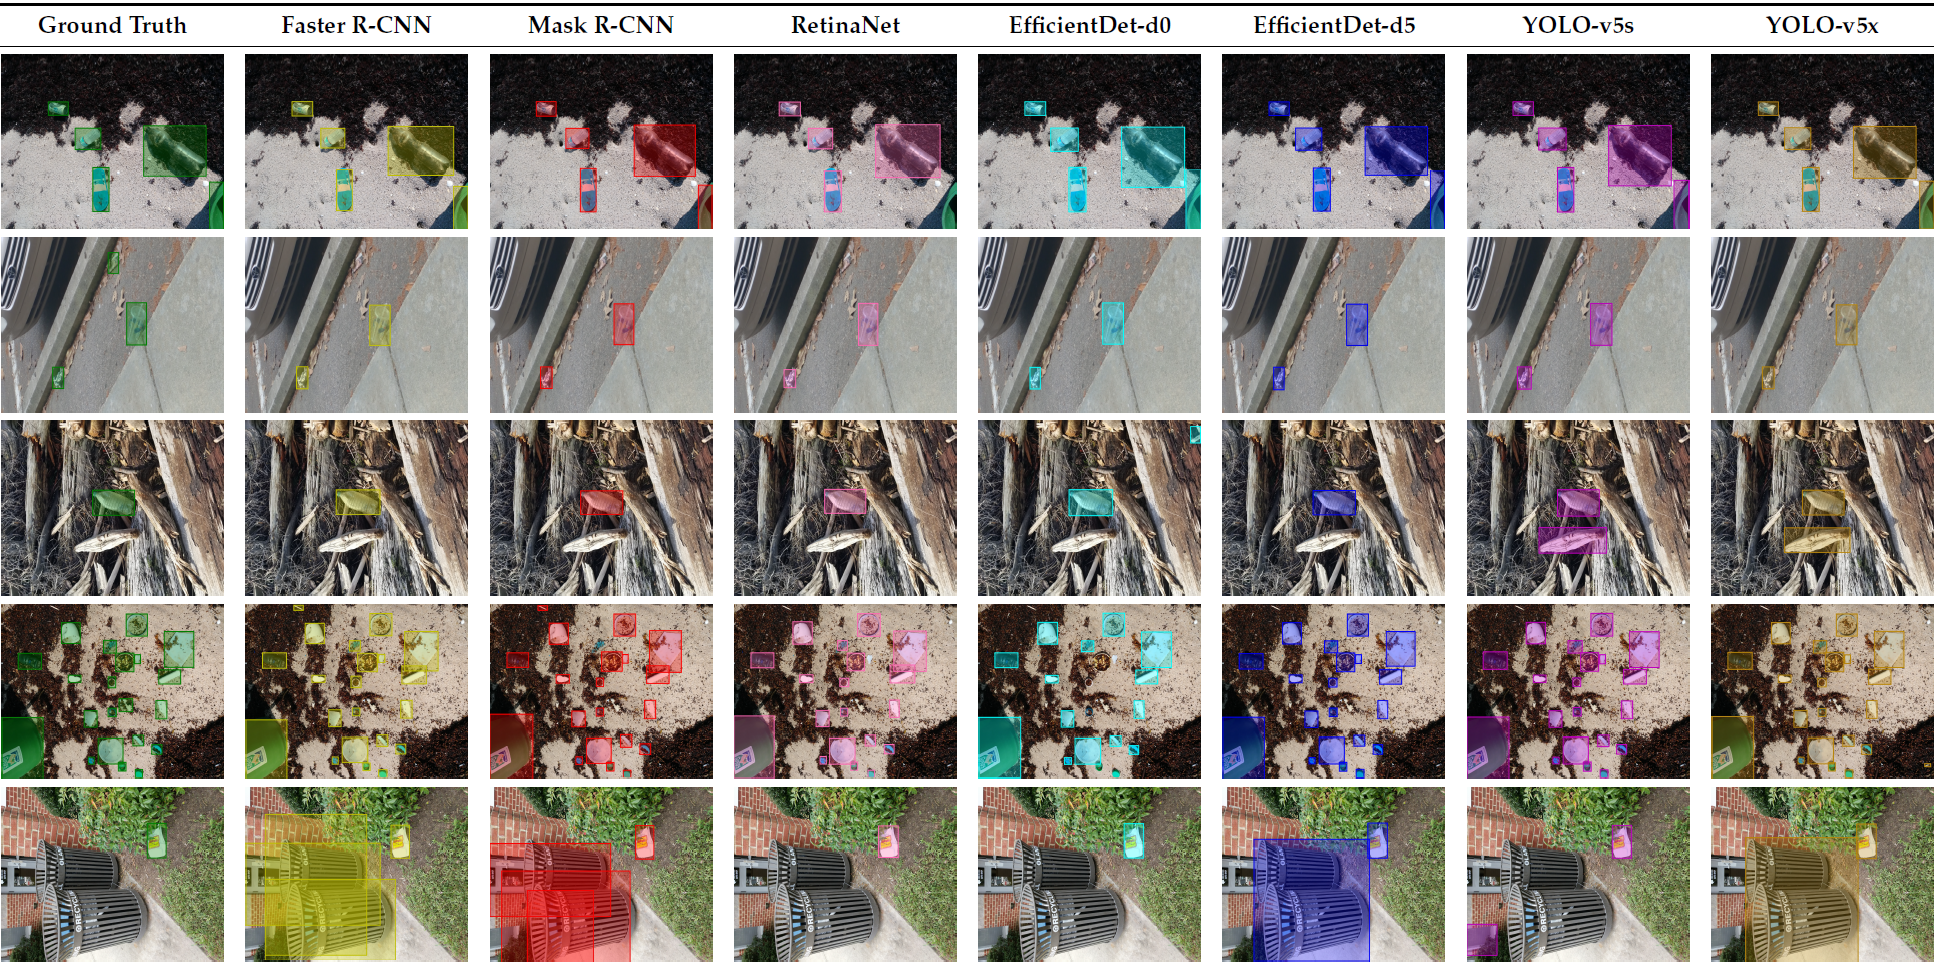
\includegraphics[width=1\linewidth]{plastopol.png}
    \caption{Visual detection results on the PlastOPol dataset. (Source: \cite{plastopol})}
    \label{fig:plastopol}
\end{figure}

To assess the performance of various deep learning models in detecting litter, the authors used both the proposed PlastOPol dataset and the publicly available \gls{taco} dataset. For the PlastOPol dataset, the data was split into 80\% for training and 20\% for testing. Evaluation metrics included \gls{ap}, \gls{map} at \gls{iou} threshold 0.5, F1-score, and recall. The models tested included EfficientDet, Faster \gls{rcnn}, Mask \gls{rcnn}, RetinaNet, and \gls{yolo}v5. As shown in Figure \ref{fig:plastopol}, the visual detection results on the PlastOPol dataset highlight the performance of these models in identifying litter objects across different environments.
The experiment results demonstrated that \gls{yolo}v5 was the best-performing model overall. The authors also observed that \gls{yolo}v5 and EfficientDet were the fastest models, even when deployed on mobile devices. However, they noted that all methods struggled with detecting small objects, such as cigarette butts. Furthermore, \gls{yolo}v5x outperformed Faster \gls{rcnn} and Mask \gls{rcnn} in terms of speed \cite{plastopol}.

\subsection{HAIDA Dataset}
\label{subsec:3_haida}

In 2022, Y.-H. Liao and J.-G. Juang developed a marine trash detection system using \gls{uav}s, aiming to replace manual efforts with UAVs for efficient marine trash detection and to provide real-time information on pollution to government agencies \cite{haida}. The real-time UAV trash monitoring system consisted of nine components: UAVs, a message queuing system, a database, a video streaming server, a connector, a UAV control station, a web service, a UAV map, and a data analysis module, as illustrated in Figure \ref{fig:haida1}. The ground station incorporated key elements, such as the video streaming server, Kafka, the Kafka connector, MongoDB, and the web service. The system addressed two key challenges: object detection and geolocation, and as part of the system's development, the authors introduced the HAIDA dataset. This dataset, collected on the NTOU campus, was used to train the object detection model and contains two types of litter objects: \textit{garbage} and \textit{bottles}. The data was gathered using a UAV equipped with a Pixhawk controller and an NVIDIA Jetson Xavier NX. The UAV operated at altitudes ranging from 1 to 10 metres \gls{agl} \cite{haida}.

\begin{figure}[!htbp]
    \centering
    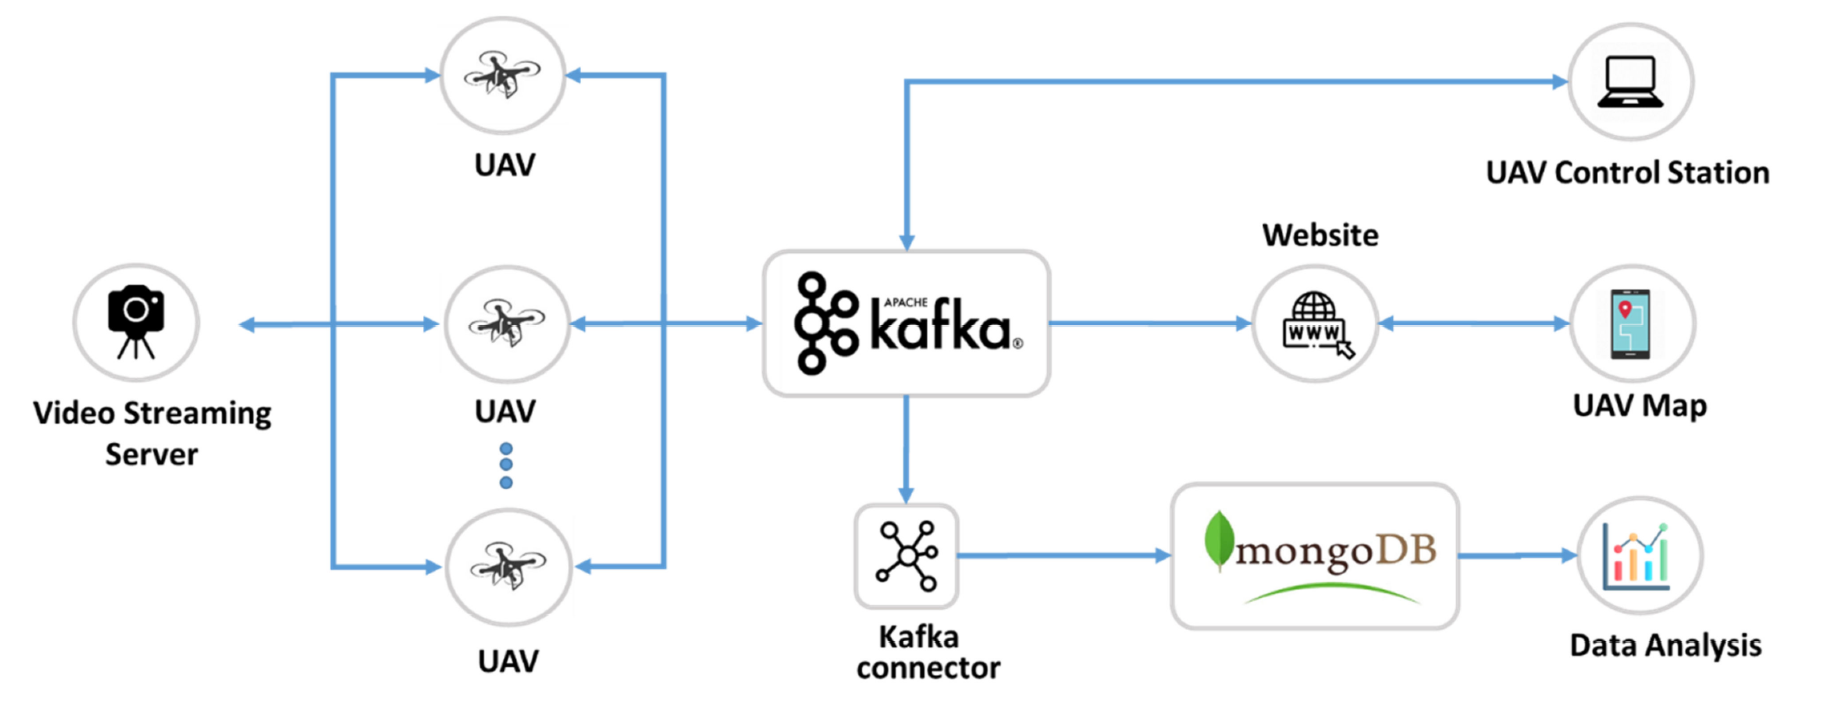
\includegraphics[width=0.7\linewidth]{haida1.png}
    \caption{The system architecture of the real-time \gls{uav} trash monitoring system. (Source: \cite{haida})}
    \label{fig:haida1}
\end{figure}

The HAIDA dataset comprises 1,319 annotated images, with 6,475 instances of litter, including 3,904 garbage objects and 2,571 bottle objects. Additionally, 456 images in the dataset contain no litter. The authors utilised the dataset to train the \gls{yolo} object detection model (version unspecified). The results showed that the model was able to identify trash objects with an \gls{ap} of over 70\% at a 0.5 \gls{iou} threshold. Notably, as shown in Figure \ref{fig:haida2}, the detection confidence for small objects was high, with confidence scores of 98.27\%, 64.65\%, and 91.86\% for different categories of litter.
The real-time UAV trash monitoring system operated by first collecting UAV footage as the drone flew across predetermined waypoints. The footage was then transmitted to a server via Kafka, where it was stored in an online database such as Oracle, MySQL, or MongoDB. Using this stored data, the server applied the trash detection model to identify litter both in the images and on a map. Control stations, both mobile and desktop, could make requests to the server to retrieve the map data, which displayed the locations of detected litter \cite{haida}.

\begin{figure}[!htbp]
  \centering
  \begin{tabular}{cc}
    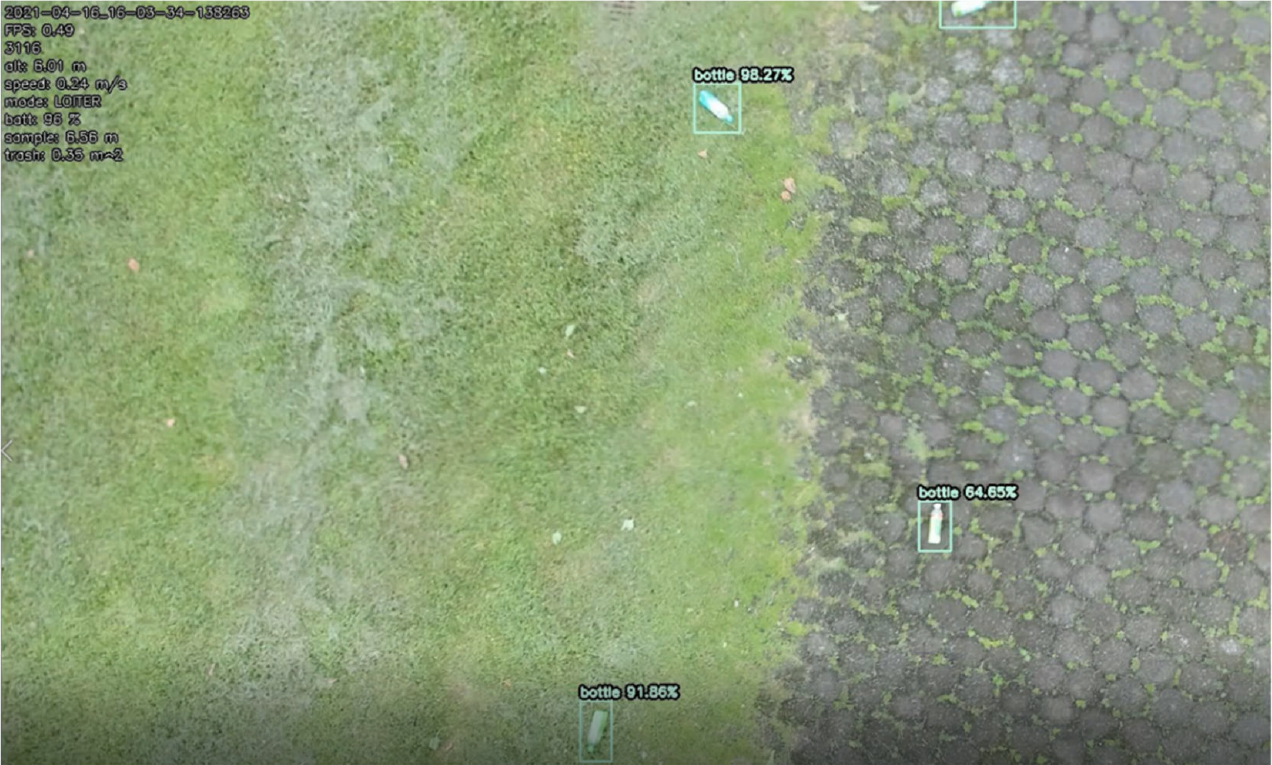
\includegraphics[width=0.48\textwidth, height=5cm]{haida2.png} &
    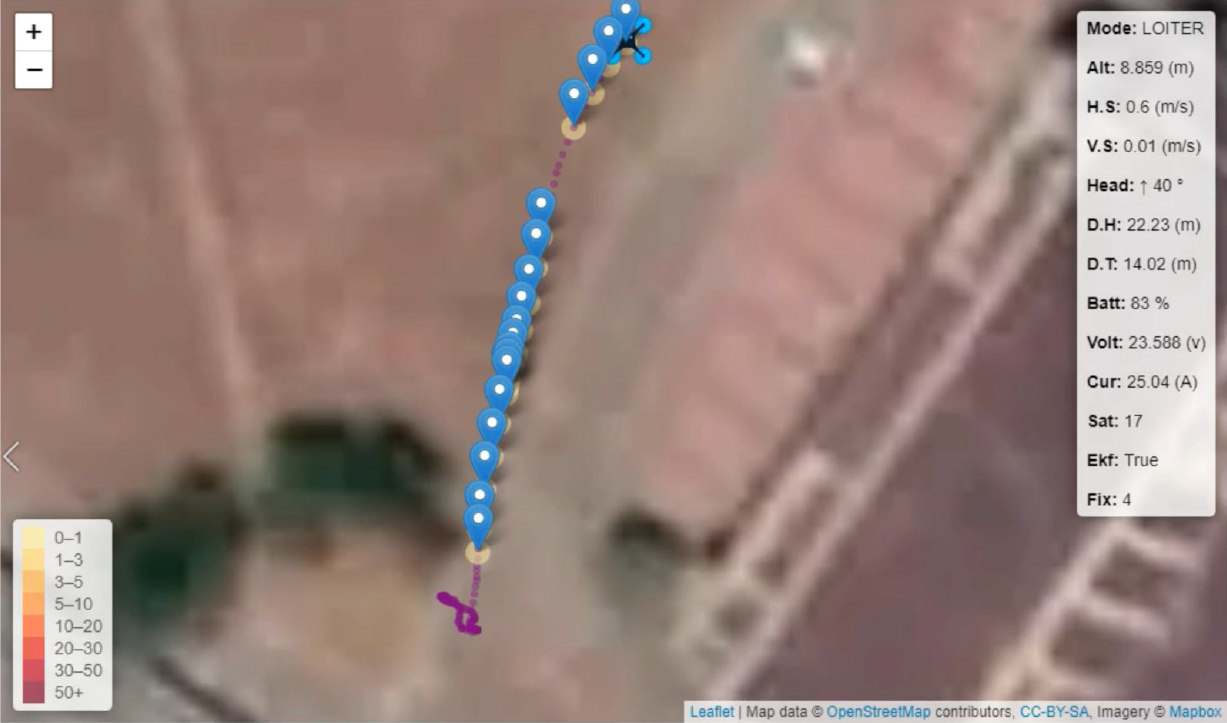
\includegraphics[width=0.48\textwidth, height=5cm]{haida3.png} \\
    \small (a) & \small (b) \\
  \end{tabular}\\
  \caption{\gls{uav} trash monitoring results on the NTOU campus. (a) Detection results from the UAV. (b) Detected litter plotted on a map, showing real-time monitoring and detection. (Source: \cite{haida})}
  \label{fig:haida2}
\end{figure}

To tackle the problem of litter geolocation, the authors adapted a similar approach to the one described in \cite{uavvaste}, enabling the calculation of the detected trash pollution area based on several factors. These factors include the camera’s horizontal and vertical angle of view, the UAV’s altitude, the camera's field of view, the dimensions of the camera's image, the size of the detected trash in the image, and the detected trash's area in both the image and the real-world environment. By incorporating these variables, the system can accurately estimate the location and extent of trash pollution in the area \cite{haida}.

\subsection{Bangladeshi Dataset}
\label{subsec:3_bangladeshi}

As populations in underdeveloped nations continue to grow, the challenges associated with trash production and disposal have become more urgent. Aware of the time-consuming and potentially hazardous nature of manual litter classification, D. Das et al. (2023) aimed to tackle this issue by developing automated methods for more efficient and safer waste management \cite{bangladeshi}. To achieve this, they focused on collecting data that accurately captured the complexities of litter in Bangladesh, creating an outdoor dataset, and incorporating OpenLitterMap to broaden its scope. This dataset comprises images from natural settings, not UAV-based data, and includes ten categories of litter: \textit{tissue paper}, \textit{plastic}, \textit{medical waste}, \textit{rope}, \textit{paper}, \textit{cigarette butts and boxes}, \textit{metal}, \textit{glass}, \textit{organic waste}, and \textit{textiles}. Initially consisting of 1,283 annotated images, the dataset was expanded to 4,418 by integrating data from OpenLitterMap, a global database containing litter and plastic images. The Bangladeshi dataset contains 6,178 instances of litter, which was extended to 8,077 while retaining the ten distinct classes \cite{bangladeshi}.

\begin{figure}[!htbp]
  \centering
  \begin{tabular}{c}
    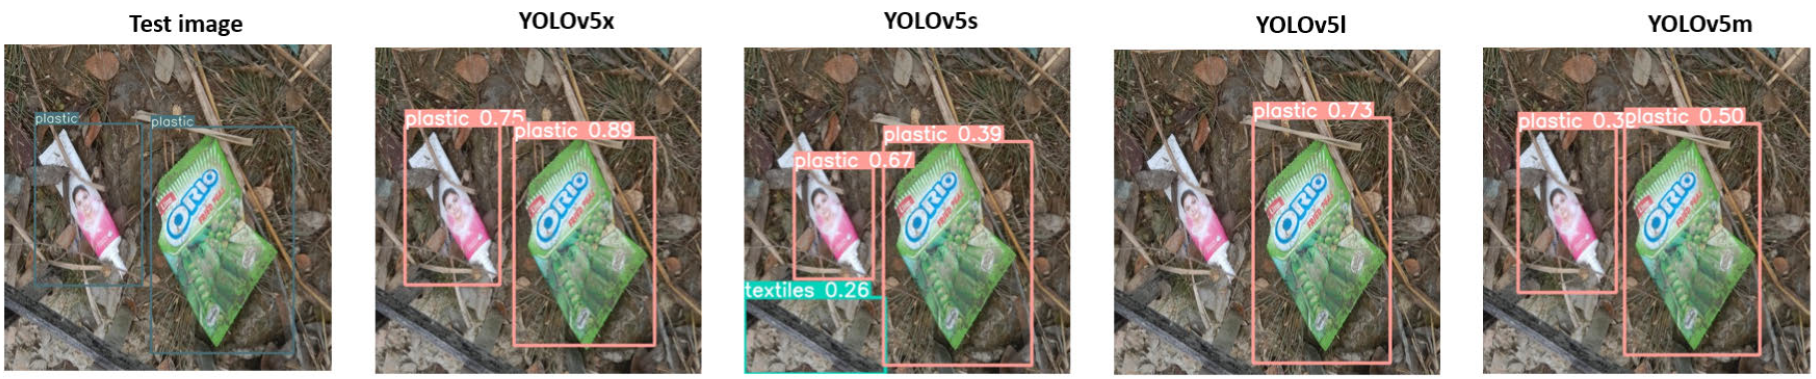
\includegraphics[width=1\textwidth]{bangladeshi1.png} \\
    \small (a)\\
    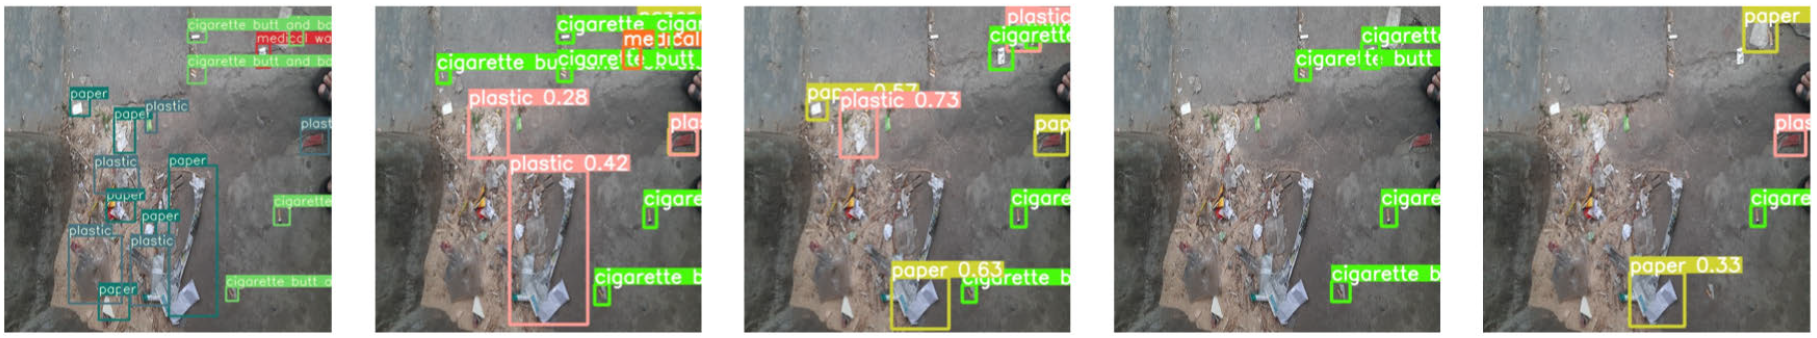
\includegraphics[width=1\textwidth]{bangladeshi2.png} \\
    \small (b) \\
  \end{tabular}\\
  \caption{Litter detection results using different versions of the \gls{yolo}v5 model on the Bangladeshi dataset. (a) 2 instances of litter; (b) 17 instances of litter. (Source: \cite{bangladeshi})}
  \label{fig:bangladeshi}
\end{figure}

The experimental setup used for this study involved a comparison with the \gls{taco} and PlastOPol datasets. The Bangladeshi dataset was divided as follows: 80\% for training, 10\% for validation, and 10\% for testing. The evaluation metrics included \gls{ap} and \gls{map} at \gls{iou} thresholds from 0.5 to 0.95, as well as F1-measure and recall. Several models were tested, including different versions of \gls{yolo}v5, \gls{yolo}v6, \gls{yolo}v8, and Faster \gls{rcnn}. The authors also employed data augmentation techniques during training and optimised model performance by adjusting hyperparameters.
In their study, the authors reported that \gls{yolo}v5x was the best-performing model, as visually demonstrated in Figure \ref{fig:bangladeshi}, which shows a comparison of the detection bounding boxes on the images, demonstrating the improved \gls{map} for the expanded dataset. However, single-class detection experiments on the \gls{taco} and PlastOPol datasets yielded better results compared to the Bangladeshi dataset. D. Das et al. also highlighted that in future work, they plan to expand the dataset to include a broader range of categories, such as ocean waste, which is currently absent. Additionally, other object detection methods, such as \gls{ssd}, Mask \gls{rcnn}, and EfficientDet, could also be evaluated using their dataset \cite{bangladeshi}.

\subsection{Beach Litter Dataset}
\label{subsec:3_beach_litter}

In 2023, R. Pfeiffer et al. proposed a framework for an autonomous beach litter monitoring and retrieval system based on drone surveys and object detection using deep learning techniques \cite{beach_litter}. Their research combined drone footage collected from the islands of Malta and Gozo, Sicily (Italy), and the Red Sea coast with publicly available litter datasets, which were subsequently used to train an object detection model for identifying litter in the captured footage. Figure \ref{fig:beachlitter1} illustrates the overall framework of the proposed beach litter monitoring system. To address both object detection and geolocation challenges, the authors compiled a \gls{uav} dataset collected with DJI Phantom 4 Pro 2.0 and DJI Mavic 2 UAVs. The dataset covered altitudes ranging from 10 metres above ground level to 60 metres above sea level and included 67 types of litter, which were categorised into seven meta-classes: \textit{clothing \& fabric}, \textit{glass}, \textit{small objects}, \textit{metal litter}, \textit{paper \& cardboard}, \textit{plastic}, and \textit{other waste}.
Additionally, the Beach Litter Dataset contains 4,126 annotated images and 10,611 litter instances, including 1,154 images with no litter present. The dataset was divided as follows: 60\% for training, 20\% for validation, and 20\% for testing. The models were evaluated using metrics such as \gls{ap},\gls{map} (at 0.5–0.95), F1-measure, and recall, with the \gls{yolo}v5 model being the primary model used for training \cite{beach_litter}. 

\begin{figure}[!htbp]
    \centering
    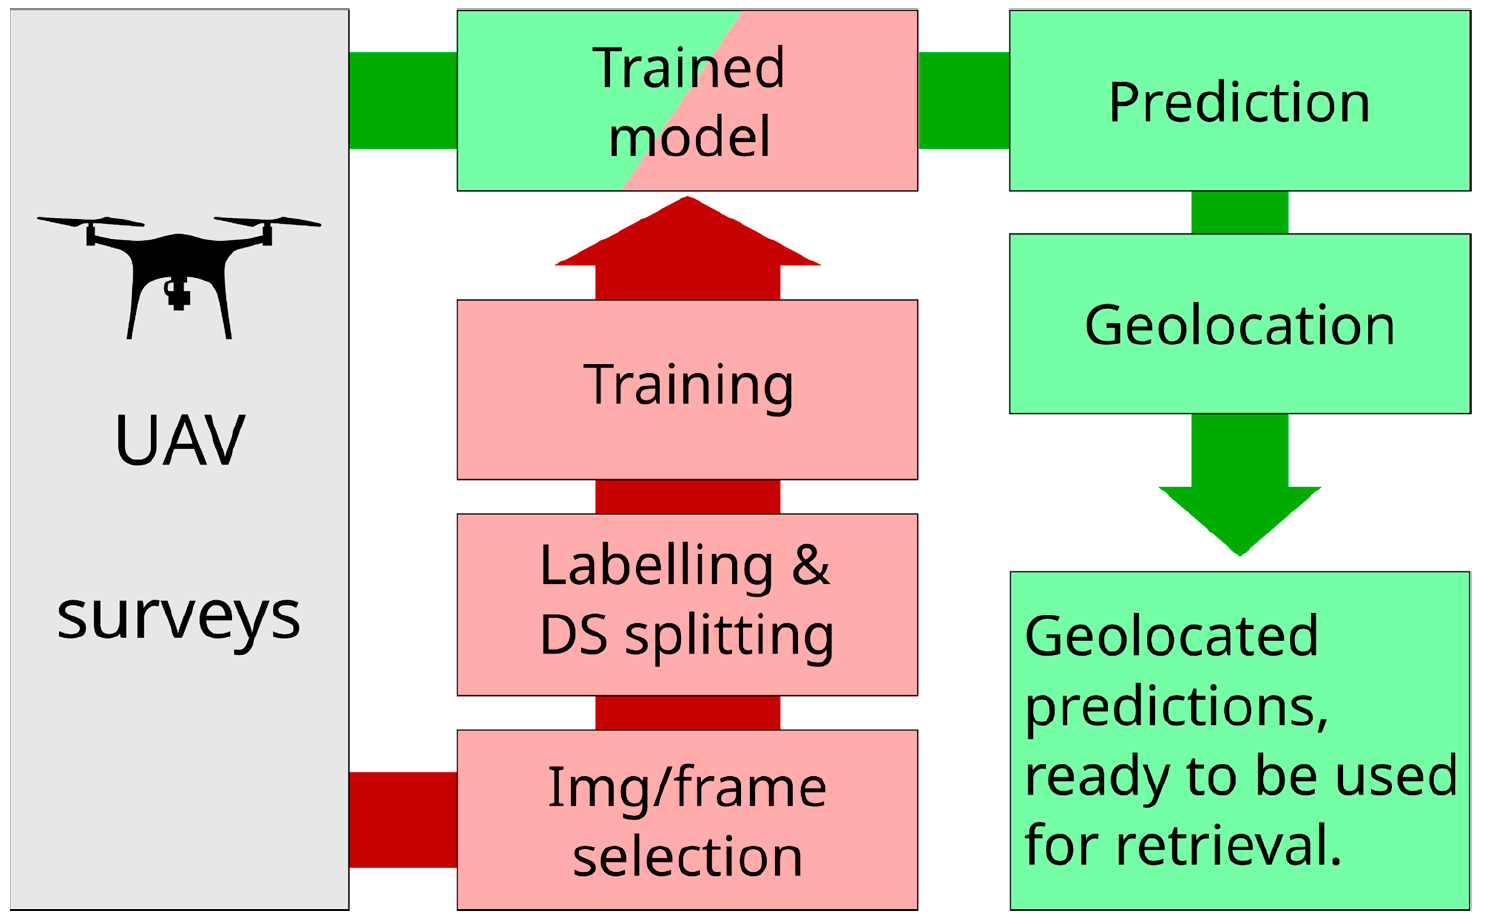
\includegraphics[width=0.7\linewidth]{beachlitter1.png}
    \caption{The system architecture of the real-time \gls{uav} beach litter monitoring and geolocation system, highlighting the two main pipelines: training (in red) and prediction (in green). (Source: \cite{beach_litter})}
    \label{fig:beachlitter1}
\end{figure}

The authors also developed a geolocation algorithm to enhance the utility of the detected litter by integrating it with a robot for debris retrieval. For the algorithm to communicate the detection coordinates to the robot, the predictions made by the \gls{yolo}v5 model needed to be geolocated. This required that the original footage include \gls{gps} coordinates of the drone. The geolocation process involved several key steps: calculating the pixel size of the footage, determining the distance between meridians and parallels at the latitude of recording, measuring the horizontal and vertical distance from the prediction box's centre to the image centre, and transforming these distances into real-world coordinates. Figure \ref{fig:beachlitter2} shows the schematic for calculating litter geolocations, highlighting the parameters used to map the detected litter to real-world coordinates. To improve accuracy, the authors also calculated the distance between each litter object and the camera’s field of view, factoring in variables such as the \gls{uav}’s height and the angle of the camera’s lens. This enabled precise localisation of litter in both the image and the real-world environment, essential for guiding the robot to specific debris \cite{beach_litter}.

\begin{figure}[!htbp]
    \centering
    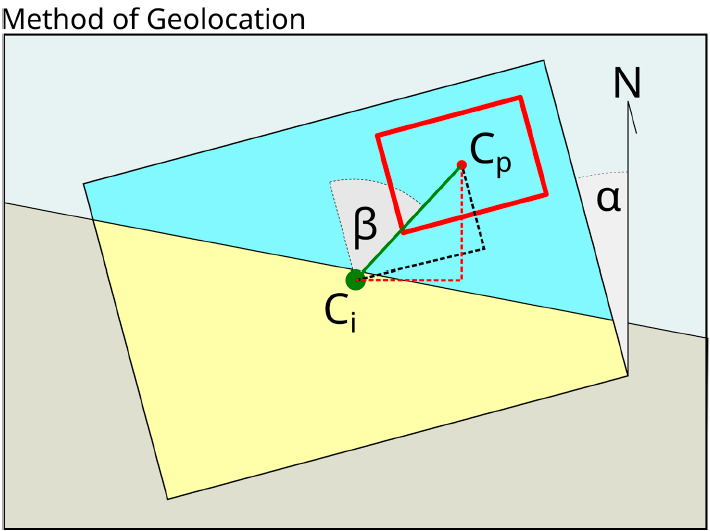
\includegraphics[width=0.7\linewidth]{beachlitter2.png}
    \caption{Schematic representation of the calculation of litter geolocations, illustrating the parameters used to map the detected litter to real-world coordinates. (Source: \cite{beach_litter})}
    \label{fig:beachlitter2}
\end{figure}

The results of their experiments using the \gls{yolo}v5 model on the labelled dataset were as follows: precision of 0.695, recall of 0.288, mAP@50 of 0.314, and mAP@50-95 of 0.2. The model performed most reliably on the following ten classes: \textit{plastic bottle}, \textit{metal can}, \textit{plastic bottle} \textit{cap}, \textit{plastic container}, \textit{shoe}, \textit{cardboard}, \textit{pop tab}, \textit{rope \& string}, \textit{wood}, and \textit{glass bottle} \cite{beach_litter}.

\subsection{TrashNet}
\label{subsec:3_trashnet}

In 2024, V. Veeravadivel Santhanalakshmi, and H. Nguyen introduced TrashNet, an object detection model designed to classify images of waste in real time. The dataset employed to train the TrashNet network comprises six primary categories of litter: \textit{cardboard}, \textit{glass}, \textit{metal}, \textit{paper}, \textit{plastic}, and \textit{general waste}. This dataset, derived from an image classification dataset on Kaggle, does not utilise UAV-based data. The TrashNet dataset comprises 2,524 annotated images, each featuring a single object instance. In addition, the authors explain that the dataset was divided into three subsets for model development: 70\% for training, 20\% for testing, and 10\% for validation.
The authors utilised \gls{yolo}v5 as the object detection model and evaluated its performance using metrics such as mean \gls{map}, precision, recall, and F1-Score. 
The authors highlight that the primary aim of this study was to develop a real-time system to assist individuals in identifying the correct bin for various types of waste near rubbish disposal areas, as seen in Figure \ref{fig:trashnet}. Notably, the model successfully fulfilled this objective, achieving an accuracy of 90\% on both the validation and testing sets \cite{trashnet}.

\begin{figure}[!htbp]
    \centering
    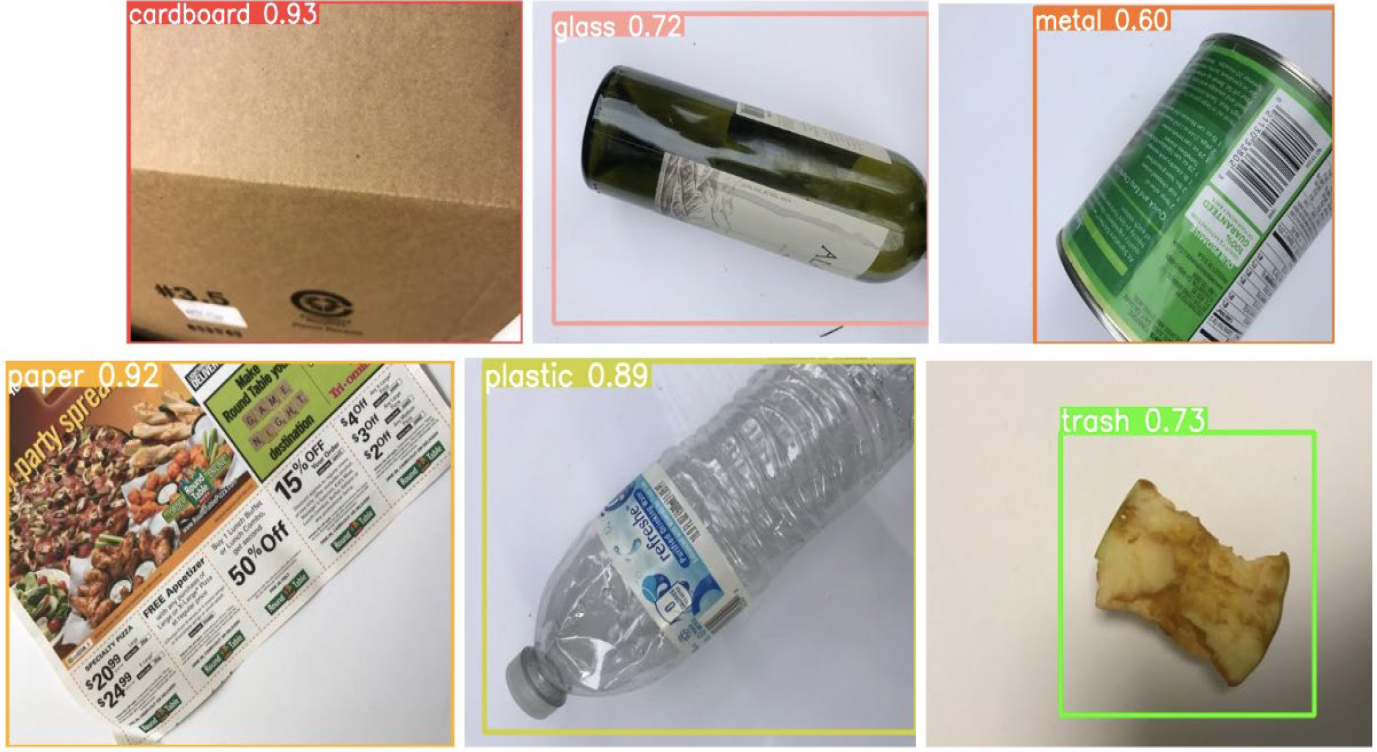
\includegraphics[width=0.7\linewidth]{trashnet.png}
    \caption{Litter detection results generated by the TrashNet detection model. (Source: \cite{trashnet})}
    \label{fig:trashnet}
\end{figure}

\subsection{SODA Dataset}
\label{subsec:3_sodadataset}

Modern \gls{uav}s are equipped with high-resolution cameras capable of capturing detailed pictures and videos of their surroundings. However, when the \gls{uav} is flying at higher altitudes, objects in the images may look very tiny, occupying only a few pixels. This poses substantial hurdles for spotting such objects. To tackle this issue, D. Pisani et al. (2024) introduced the \gls{soda} dataset, designed to aid research focused on small object detection in aerial imagery \cite{soda_dataset}. The dataset features six primary types of litter, derived from the \gls{taco} dataset: \textit{clear plastic bottles}, \textit{other plastic bottles}, \textit{glass bottles}, \textit{glass jars}, \textit{drinking cans}, and \textit{drinking cartons}. Figure \ref{fig:soda1} illustrates examples of litter categories used in the \gls{soda} dataset. Furthermore, the images were collected using a combination of DJI Mini 2 and DJI Air 2S UAVs at various altitudes, including 1m, 5m, 10m, 15m, 20m, 25m, and 30m \cite{soda_dataset, detect_litter}.

\begin{figure}[!htbp]
    \centering
    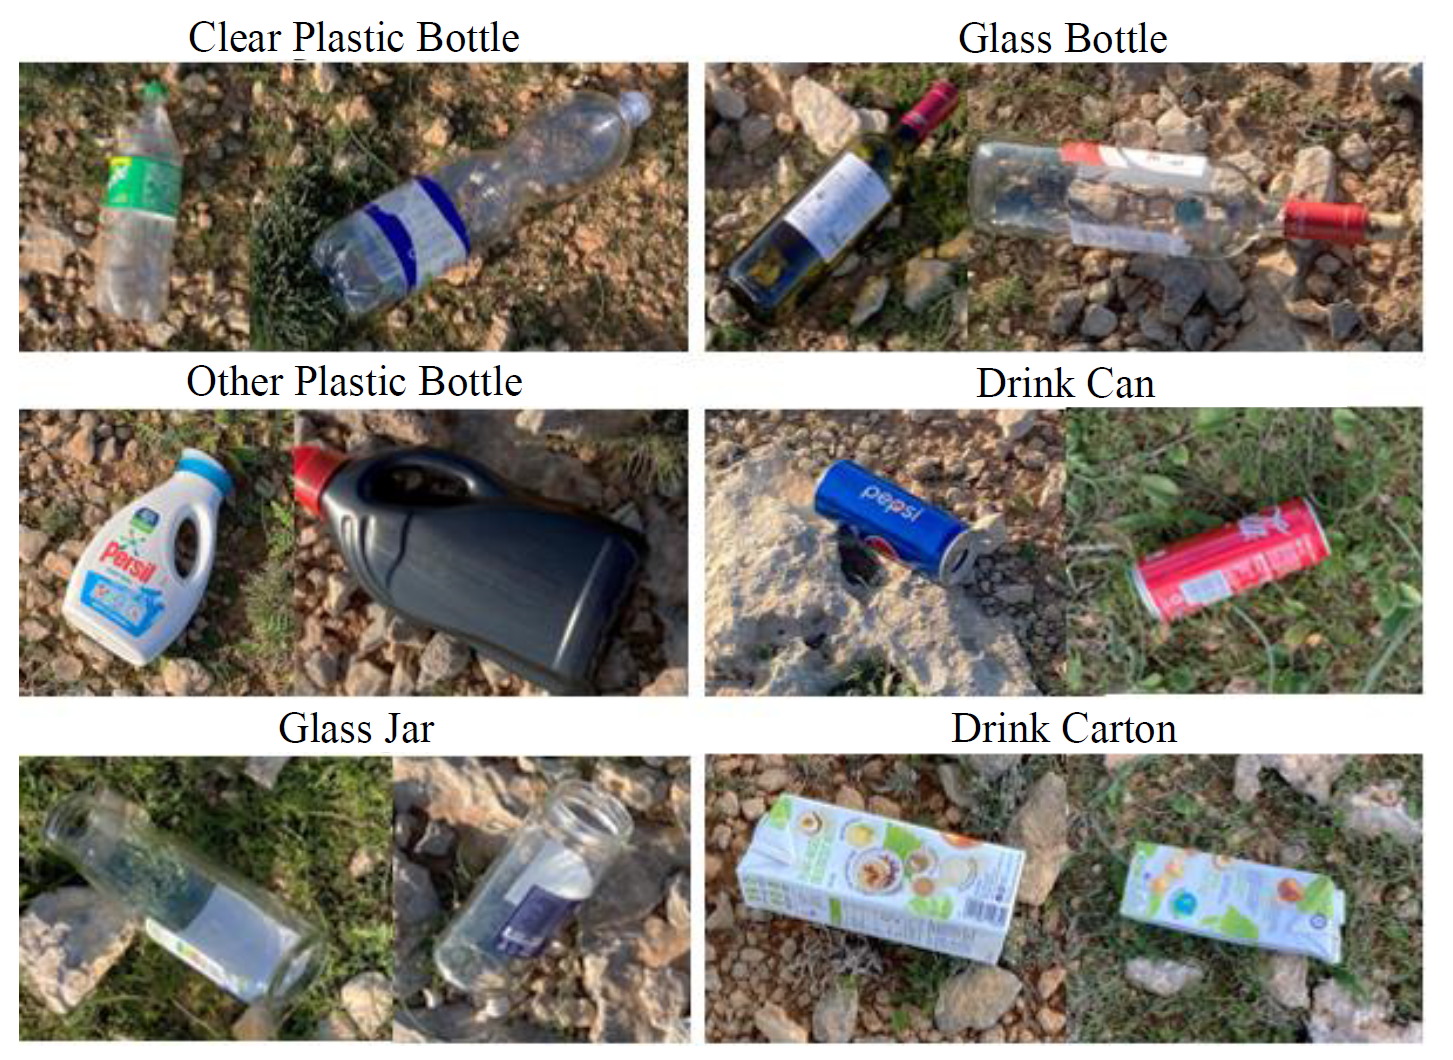
\includegraphics[width=0.8\columnwidth]{soda_images.png}
    \caption{The six object categories featured in the SODA dataset. (Source: \cite{soda_dataset})}
    \label{fig:soda1}
\end{figure}

The \gls{soda} dataset consists of 829 annotated images, with 452 (54.52\%) taken at 1 metre and 377 (45.48\%) captured from altitudes of 5 metres or more. 
The \gls{soda} dataset supports multi-class classification, with each object annotated with a distinct label using polygons rather than bounding boxes. The authors explain that polygons offer a more accurate fit around the object, whereas bounding boxes often capture additional background. Additionally, they clarify that polygons provide precise alignment during augmentations, such as rotation. Techniques for annotating with polygons and applying these augmentations are outlined in \cite{mask_to_annotation}. However, although the \gls{soda} dataset is annotated using polygons, the authors focus on the challenge of object detection rather than instance segmentation.
To address the challenge of detecting small objects across multiple categories of litter, the authors employed three different training strategies. The first approach involved segregating the training dataset according to altitude. In the second approach, the dataset was merged while maintaining multi-class labels. The third approach also merged the dataset but consolidated all categories into a single \textit{litter} class. 
Notably, a key feature of this study was the application of a \textit{tiling methodology} to improve the detection of small objects. This technique divides an image into a grid and splits it into smaller, equally sized sections, which were used in both the training and inference stages. The authors note that the grid size can significantly influence detection performance, with smaller grids, such as $2 \times 2$ (refer to Figure \ref{fig:soda2}), used at lower altitudes and larger grids, like $5 \times 5$, applied at higher altitudes. For the \gls{soda} dataset, a $5 \times 5$ grid was used across all altitudes and images \cite{detect_litter, soda_dataset, daniel_thesis}.

\begin{figure}[!htbp]
    \centering
    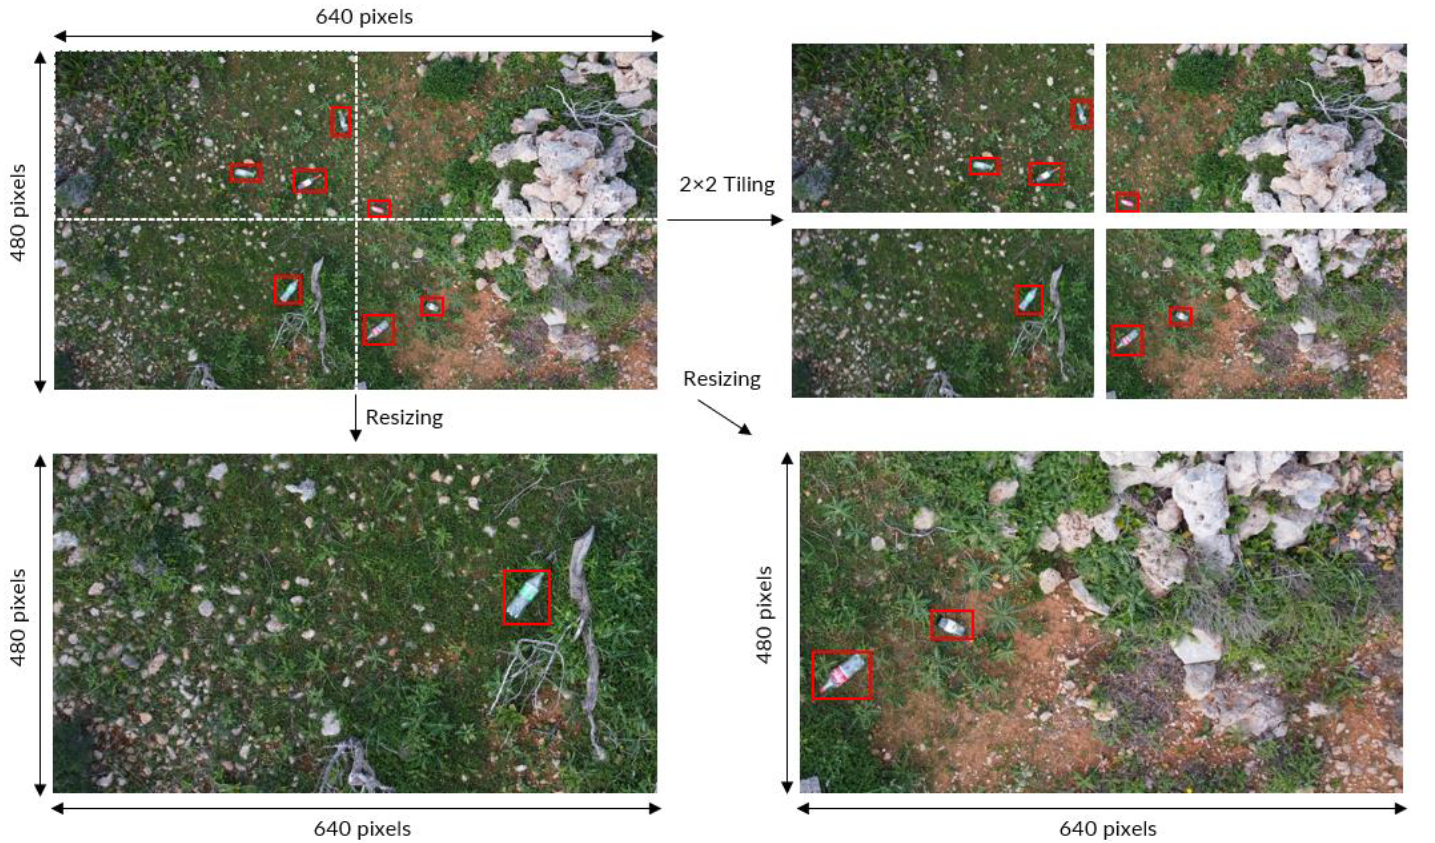
\includegraphics[width=0.9\columnwidth]{soda2.png}
    \caption{Application of a $2 \times 2$ tiling grid to aerial imagery captured at an altitude of 5 metres. (Source: \cite{detect_litter})}
    \label{fig:soda2}
\end{figure}

Three object detection models were trained for this study: \gls{yolo}v5 and \gls{yolo}v8 (both one-stage detectors) and Faster \gls{rcnn} (a two-stage detector). Models trained using the second and third approaches were evaluated on the \gls{bdw} dataset. The results indicated that the third approach, which merged all classes into a single litter category, outperformed the second approach. Additionally, the evaluation revealed that the \gls{soda} dataset was lacking a sufficient number of images of clear plastic bottles. 
In terms of \gls{map}, the results for the different models were as follows: Faster \gls{rcnn} achieved a \gls{map} of 0.921, \gls{yolo}v5 had a \gls{map} of 0.854, and \gls{yolo}v8 performed with a \gls{map} of 0.728 \cite{soda_dataset, detect_litter}. 

Finally, this study contributes to the use of \gls{uav}s for capturing aerial imagery and applying computer vision techniques to detect and classify objects within these images. The authors emphasise its significance as a crucial phase and a stepping stone towards the automation of litter collection for cleanup efforts \cite{detect_litter, soda_dataset, daniel_thesis}.

\vspace{\baselineskip}
\noindent
Table \ref{tab:lit_review} presents a systematically organised comparison of the datasets and approaches, highlighting that the three primary challenges addressed were object detection, instance segmentation, and object geolocation, spanning both \gls{uav}-based and non-\gls{uav} datasets. It is also evident that for \gls{uav}-based approaches, altitudes ranging from 10 metres to 30 metres were the most commonly used. Additionally, in terms of the number of categories or litter types represented across datasets, both \gls{uav} and non-\gls{uav} approaches predominantly focus on creating single-class labelled datasets, with a few exceptions, such as recent approaches employing 6 to 10 classes, excluding the Beach Litter \cite{beach_litter} and \gls{taco} \cite{taco2020} datasets. Additionally, despite non-UAV datasets often containing a relatively large number of images, most \gls{uav}-based datasets consist of a smaller number of images, with notable exceptions being the \gls{bdw} \cite{bdwdataset} and Beach Litter \cite{beach_litter} datasets.

\begin{table*}[htbp]
\centering
\scriptsize
\hspace*{-0.5in} % Adjust this value to shift the table leftward
\begin{tabular}{|l|c|c|c|c|c|l|}
\hline
\textbf{Name} & \textbf{Year} & \textbf{No of. Images} & \textbf{UAV Approach} & \textbf{AGL Altitudes} & \textbf{Problems} & \textbf{No of. Categories} \\ 
\hline \hline
BDW Dataset \cite{bdwdataset} & 2018 & 25,407 & Yes & 10m--30m & Detection & 1 (Litter) \\ \hline
UM Geo. Survey \cite{umgeosurvey} & 2018 & 472 & Yes & 30m & Data Collection & 5 (Litter) \\\hline
SuperDock \cite{superdock} & 2019 & 100 & Yes & 5m--10m & Detection & 1 (Litter) \\\hline
Styrofoam Monitoring \cite{styrofoam} & 2019 & N/S & Yes & 15m & Detection, Segmentation & 1 (Litter) \\\hline
Small Litter Detection \cite{small_litter_detection} & 2019 & 744 & Yes & 5m--10m & Detection & 1 (Litter) \\\hline
TACO Dataset \cite{taco2020} & 2020 & 1,500 & No & N/A & Detection, Segmentation & 60 (Litter) [28 Super] \\\hline
MJU-Waste Dataset \cite{mju_waste} & 2020 & 2,475 & No & N/A & Segmentation & 1 (Litter) \\\hline
UAVVaste Dataset \cite{uavvaste} & 2021 & 772 & Yes & low-altitude & Detection, Geolocation & 1 (Litter) \\\hline
ZeroWaste Dataset \cite{zerowaste} & 2022 & 10,715 & No & N/A & Detection, Segmentation & 4 (Litter) \\\hline
PlasOPol Dataset \cite{plastopol} & 2022 & 2,418 & No & N/A & Detection & 1 (Litter) \\\hline
HAIDA Dataset \cite{haida} & 2022 & 1,319 & Yes & 1m--10m & Detection, Geolocation & 2 (Litter) \\\hline
Bangladeshi Dataset \cite{bangladeshi} & 2023 & 4,418 & No & N/A & Detection & 10 (Litter) \\\hline
Beach Litter Dataset \cite{beach_litter} & 2023 & 4,126 & Yes & 10m--60m & Detection, Geolocation & 67 (Litter) [7 Super] \\\hline
TrashNet \cite{trashnet} & 2024 & 2,524 & No & N/A & Detection & 6 (Litter) \\\hline
SODA Dataset \cite{soda_dataset} & 2024 & 829 & Yes & 1m, 5m--30m & Detection, Segmentation & 6 (Litter) [4 Super] \\\hline
\end{tabular}
\caption{Comparison of datasets and approaches, systematically organised, with litter-related images captured from both \gls{uav} and non-\gls{uav} data.}
\label{tab:lit_review}
\end{table*}

\section{Learning Using Privileged Information in Computer Vision}
\label{subsec:2_lupi}
\gls{lupi}
The Learning using Privileged Information (LUPI) paradigm, introduced by V. Vapnik and A. Vashist \cite{lupi, Vapnik2015LearningUP}, expands traditional learning tasks by incorporating supplementary data alongside the standard input/output training pairs in machine learning. This additional information is often more pertinent to the task at hand, thereby improving prediction accuracy. The concept of LUPI allows for the \textit{transfer of knowledge} from a teacher, trained with privileged data, to a student who only has access to the input information.
In the field of Computer Vision, several problems present an asymmetric distribution of information between training and test phases \cite{learning2rank}, making LUPI particularly applicable. V. Sharmanska et al. \cite{learning2rank} investigate four types of privileged information for object classification: semantic properties, bounding boxes, tags, and annotator rationale. Their study shows that applying LUPI to the SVM+ algorithm improves performance.
In a similar study, S. Wang et al. \cite{lupi_classification} address the same issue by applying similarity constraints to capture the relationship between available and privileged information. The authors use high-resolution images and image tags as privileged data, which are accessible during training but not during testing.

\section{Knowledge Distillation in Computer Vision}
\label{subsec:2_distillation}
Knowledge distillation is a pivotal technique in machine learning that allows the transfer of knowledge from a large, complex model to a smaller, more efficient one. In the context of computer vision, as discussed by \cite{distillation1}, there are various methods for achieving this, including response-based, feature-based, and relation-based knowledge transfer. These approaches can be applied across a wide range of vision tasks, such as image classification, object detection, and multimodal vision models \cite{distillation1}. Focusing on object detection, two common distillation techniques are feature imitation and logit mimicking \cite{distillation2}. Interestingly, the use of valuable localisation regions to selectively distil both classification and localisation knowledge for specific areas is another key aspect of this process, as proposed in \cite{distillation2}.
feature-based and representation-based


\section{Conclusion}
\label{sec:3_conclusion}